% ==========================================================================
%  Bachelor Thesis — Explainable AI in Multi-Tenant ERPs:
%                    Navigating Data Sparsity and the Cold-Start Problem
%
%  Build with:  latexmk -pdf sparsity_thesis.tex
%  Bibliography: natbib + plainnat, references_sparsity.bib
% ==========================================================================
\documentclass[12pt,a4paper,oneside]{report}

% ── Encoding / language ───────────────────────────────────────────
\usepackage[utf8]{inputenc}
\usepackage[T1]{fontenc}
\usepackage{times}
\usepackage[english]{babel}

% ── Page layout ───────────────────────────────────────────────────
\usepackage[a4paper,top=3cm,bottom=3cm,left=4cm,right=3cm]{geometry}
\usepackage{setspace}
\onehalfspacing

% ── Graphics / figures / tables ───────────────────────────────────
\usepackage{graphicx}
\graphicspath{{figures/}{results/sparsity_experiment/figures/}{results/hr_attrition_experiment/figures/}{results/lead_scoring_experiment/figures/}}
\usepackage{float}
\usepackage{caption}
\usepackage{subcaption}
\usepackage{booktabs}
\usepackage{longtable}
\usepackage{array}
\usepackage{tabularx}
\usepackage{multirow}

% ── Lists / code / colour ─────────────────────────────────────────
\usepackage{enumitem}
\usepackage{xcolor}
\usepackage{listings}
\definecolor{codebg}{RGB}{248,248,248}
\definecolor{codecomment}{RGB}{106,153,85}
\definecolor{codekeyword}{RGB}{0,0,180}
\definecolor{codestring}{RGB}{163,21,21}
\lstdefinestyle{pystyle}{
  language=Python,
  basicstyle=\ttfamily\footnotesize,
  backgroundcolor=\color{codebg},
  commentstyle=\color{codecomment}\itshape,
  keywordstyle=\color{codekeyword}\bfseries,
  stringstyle=\color{codestring},
  numbers=left, numberstyle=\tiny\color{gray},
  frame=single, framesep=4pt, rulecolor=\color{gray!40},
  breaklines=true, showstringspaces=false, captionpos=b, tabsize=2,
}
\lstset{style=pystyle}

% ── Math ──────────────────────────────────────────────────────────
\usepackage{amsmath, amssymb, amsfonts}

% ── TikZ for native diagrams (Figures 1.1, 2.3, 3.2) ──────────────
\usepackage{tikz}
\usetikzlibrary{positioning,arrows.meta,shapes.geometric,fit,calc,decorations.pathreplacing}

% ── References / hyperlinks ───────────────────────────────────────
\usepackage[round,authoryear]{natbib}
\usepackage{url}
\usepackage[hidelinks,colorlinks=false]{hyperref}
\usepackage{fancyhdr}
\usepackage{titlesec}
\usepackage{tocloft}

% ── Header / footer ───────────────────────────────────────────────
\pagestyle{fancy}
\fancyhf{}
\renewcommand{\headrulewidth}{0.4pt}
\renewcommand{\footrulewidth}{0pt}
\fancyhead[L]{\nouppercase{\leftmark}}
\fancyhead[R]{\thepage}
\fancypagestyle{plain}{\fancyhf{}\fancyfoot[R]{\thepage}\renewcommand{\headrulewidth}{0pt}}

% ── Chapter / section titling ─────────────────────────────────────
\titleformat{\chapter}[display]
  {\normalfont\Large\bfseries\centering}
  {\MakeUppercase{\chaptertitlename}\ \thechapter}{14pt}{\Large}
\titlespacing*{\chapter}{0pt}{-20pt}{30pt}

% ── Project-wide macros ───────────────────────────────────────────
\newcommand{\projecttitle}{Explainable AI in Multi-Tenant ERPs:\\Navigating Data Sparsity and the Cold-Start Problem}
\newcommand{\authorname}{Ahmed Ameen Hassan Alkuraimi}
\newcommand{\studentid}{NIM / 220535618354}
\newcommand{\advisorone}{Dr. Eng. Muhammad Ashar, S.T., M.T.}
\newcommand{\institution}{Faculty of Engineering\\State University of Malang}
\newcommand{\submissionyear}{2026}

\hypersetup{
  pdftitle={\projecttitle},
  pdfauthor={\authorname},
  pdfsubject={Explainable AI, Multi-Tenant ERP, Cold-Start Problem},
  pdfkeywords={XAI, SHAP, LIME, multi-tenant, ERP, cold-start, Django},
}

% ==========================================================================
\begin{document}
% ==========================================================================

% ── Front matter ──────────────────────────────────────────────────
\pagenumbering{roman}

% Title page
\begin{titlepage}
  \centering
  \vspace*{1cm}
  {\Large\bfseries \projecttitle\par}
  \vspace{1.5cm}
  {\large \textit{A Bachelor's Thesis}\par}
  \vspace{0.4cm}
  {\normalsize Submitted in partial fulfilment of the requirements\\for the degree of Bachelor of Computer Science\par}
  \vspace{1.2cm}
  
\includegraphics[width=0.32\textwidth]{Lambang-UM.png}\par
  \vspace{1.2cm}
  {\large \textbf{\authorname}\par}
  {\normalsize \studentid\par}
  \vspace{2cm}
  {\normalsize Supervised by\par}
  {\large \advisorone\par}
  \vfill
  {\normalsize \institution\par}
  {\normalsize \submissionyear\par}
\end{titlepage}

% Abstract
\chapter*{Abstract}
\addcontentsline{toc}{chapter}{Abstract}
\markboth{Abstract}{Abstract}

The proliferation of multi-tenant Enterprise Resource Planning (ERP) systems has democratized access to embedded Machine Learning (ML) services for Small and Medium-sized Enterprises (SMEs). Modern ERP platforms ship with predictive modules for late-payment risk, lead scoring, and employee attrition, and increasingly augment these models with post-hoc Explainable AI (XAI) techniques such as SHAP and LIME. While the data-rich enterprise regime is well served by this combination, the long tail of cold-start tenants---those with only tens or hundreds of historical records---reveals a previously under-examined failure mode: \emph{hallucinated explanations}. SHAP and LIME continue to produce confident, well-formatted attributions even when the underlying classifier is statistically equivalent to random guessing, exposing SME users to authoritative-looking but epistemically empty recommendations.

This thesis quantifies the phenomenon through a controlled sparsity experiment across five simulated tenants ($50{,}000$; $5{,}000$; $1{,}000$; $200$; $50$ rows) drawn from the Brazilian Olist e-commerce corpus, operationalised as a \emph{Late Delivery Risk} prediction task ($\mathbf{1}[\textit{delivered\_customer\_date} > \textit{estimated\_delivery\_date}]$) that serves as a structural ERP-style operational-risk substrate generalising to the studied system's late-payment module, and trained under a strict leakage-avoidance regime in which only order-time observables are admitted into the feature matrix. Classical predictive metrics fail to track the regime change: AUC-ROC remains uniformly modest across the data-rich, medium, sparse, and very-sparse tiers ($0.6556$, $0.6249$, $0.6094$, $0.6126$) and \emph{rises} anomalously to $0.8889$ at the cold-start tier as a small-sample artefact. Baseline rank agreement of SHAP explanations against the data-rich reference tenant (a reference-aligned explanation-stability measure, not a ground-truth fidelity claim), quantified by the Spearman rank correlation of global SHAP importances, drops monotonically from $\rho = 1.000$ to $\rho = 0.4485$, crossing below the $\rho = 0.70$ reliability threshold at the $1{,}000$-row mark ($\rho_C = 0.6429$). Explanation volatility, measured by the variance of absolute SHAP values, expands by more than two orders of magnitude---from $0.0224$ at the data-rich tier to $5.0392$ at the cold-start tier. The qualitative cliff is replicated under the same pipeline on two further ERP-native tasks (IBM HR Analytics Employee Attrition; synthetic CRM Lead Scoring), supporting the external validity of the architectural finding. Building on these empirical findings, the thesis proposes and implements a \textbf{Maturity-Aware AI Routing} pattern in a Django~4.2 multi-tenant ERP: a tier-logic gate (\texttt{LatePaymentPredictor.predict\_or\_heuristic}) that suppresses local predictions for tenants below the $1{,}000$-invoice threshold and substitutes platform-wide global heuristics derived from the data-rich reference. The proposed architecture provides a concrete, auditable systems-level control against hallucinated explanations and offers SaaS vendors a scalable cold-start fallback consistent with emerging AI-accountability regulation.

\noindent\textbf{Keywords:} Explainable AI, SHAP, LIME, multi-tenant SaaS, ERP, cold-start, data sparsity, Django, reliability cliff.

% Tables of contents / figures / tables
\tableofcontents
\listoffigures
\listoftables

% ── Main matter ───────────────────────────────────────────────────
\clearpage
\pagenumbering{arabic}
\setcounter{page}{1}

% !TEX root = ../sparsity_thesis.tex
\chapter{Introduction}
\label{ch:introduction}

\section{Background}
\label{sec:background}

Enterprise Resource Planning (ERP) systems have evolved over the past two decades from monolithic, on-premise installations affordable only to large corporations into cloud-delivered, multi-tenant Software-as-a-Service (SaaS) platforms accessible to small and medium-sized enterprises (SMEs). This democratization has been driven by the multi-tenant architectural model, in which a single application instance---or a single application instance coupled with isolated per-tenant databases---serves many customer organizations simultaneously, dramatically reducing the marginal cost of onboarding a new business. As a consequence, the modern ERP is no longer merely a transactional system of record for finance, sales, and human resources; it is increasingly expected to function as an analytical platform capable of forecasting late payments, scoring sales leads, and predicting employee attrition.

The mechanism through which contemporary ERP vendors deliver these analytical capabilities is machine learning (ML). Tabular classifiers such as gradient-boosted decision trees and random forests have proven highly effective at predicting business outcomes from the structured operational data that ERPs accumulate. However, these models are widely characterized as ``black boxes'': their internal decision logic is not directly interpretable by the business users who are expected to act on their outputs. In a B2B context where an algorithmic recommendation may directly influence whether credit is extended to a customer, whether a salesperson pursues a lead, or whether a manager intervenes to retain an employee, an opaque prediction is operationally unacceptable and, under emerging regulation such as the European Union's Artificial Intelligence Act, increasingly legally untenable.

The academic and industrial response to this opacity has been the rapid maturation of the field of Explainable Artificial Intelligence (XAI). Post-hoc, model-agnostic techniques---most prominently SHapley Additive exPlanations (SHAP) and Local Interpretable Model-agnostic Explanations (LIME)---have emerged as de facto standards for translating the predictions of any tabular classifier into human-readable feature attributions. The prevailing narrative in both the literature and vendor marketing positions SHAP and LIME as the architectural component that closes the loop between predictive ML and trustworthy business decision-making.

This narrative, however, has been validated almost exclusively on data-rich settings: large, mature, single-tenant enterprises whose historical record contains tens of thousands of labelled transactions. The multi-tenant SaaS ERP context is fundamentally different. In a platform serving thousands of tenants, the data volume per tenant follows a long-tail distribution: a small number of mature customers contribute the bulk of the records, while the majority of tenants---particularly newly-onboarded SMEs---operate in a persistent state of data scarcity, the so-called \emph{cold-start} regime. Under such conditions, a per-tenant ML model is trained on a handful of observations and consequently exhibits little to no genuine predictive power.

What has gone largely unexamined in the literature is the behaviour of post-hoc XAI techniques under exactly these conditions. SHAP and LIME are \emph{unconditional} explainers: they will produce a confidently-rendered, visually-compelling attribution diagram for any prediction made by any model, regardless of whether that model is actually learning a signal or merely interpolating noise. The result is a phenomenon this thesis names the \textbf{hallucinated explanation}: a polished, business-grade narrative (``This invoice is at risk of late payment primarily because of \texttt{payment\_value} and \texttt{freight\_value}'') that is generated with full visual authority on top of a model whose discriminative performance is statistically indistinguishable from random guessing. For the cold-start SME tenant, the XAI layer that was supposed to function as a trust-building safeguard becomes, instead, a mechanism for the systematic manufacture of false confidence.

\begin{figure}[h]
    \centering
    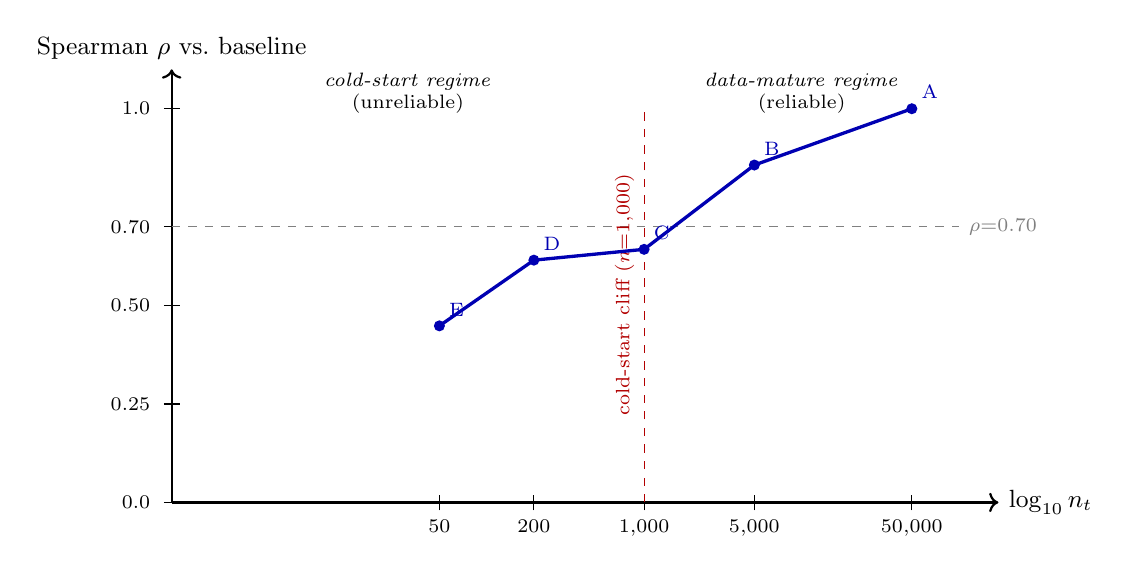
\begin{tikzpicture}[x=1.0cm,y=1.0cm]
        % Axes
        \draw[->,thick] (0,0) -- (10.5,0) node[right] {\small $\log_{10} n_t$};
        \draw[->,thick] (0,0) -- (0,5.5) node[above] {\small Spearman $\rho$ vs.\ baseline};
        % y-axis ticks
        \foreach \y/\lab in {0/0.0, 1.25/0.25, 2.5/0.50, 3.5/0.70, 5/1.0} {
            \draw (-0.1,\y) -- (0.1,\y);
            \node[left,font=\scriptsize] at (-0.15,\y) {\lab};
        }
        % x-axis ticks at tenant tiers: log10(50)=1.7, log10(200)=2.3, log10(1000)=3, log10(5000)=3.7, log10(50000)=4.7
        \foreach \x/\lab in {1.7/{50}, 2.3/{200}, 3/{1{,}000}, 3.7/{5{,}000}, 4.7/{50{,}000}} {
            \draw (\x*2,-0.1) -- (\x*2,0.1);
            \node[below,font=\scriptsize] at (\x*2,-0.1) {$\lab$};
        }
        % Reliability threshold rho = 0.70
        \draw[dashed,gray] (0,3.5) -- (10,3.5);
        \node[gray,font=\scriptsize,right] at (10,3.5) {$\rho{=}0.70$};
        % Cold-start cliff vertical at n=1000 (x = 3*2 = 6)
        \draw[dashed,red!70!black] (6,0) -- (6,5);
        \node[red!70!black,font=\scriptsize,above,rotate=90] at (6,2.5) {\quad cold-start cliff ($n{=}1{,}000$)};
        % Empirical curve through (1.7,2.24)=E, (2.3,3.08)=D, (3,3.21)=C, (3.7,4.28)=B, (4.7,5)=A
        % rho: A=1.00, B=0.857, C=0.6429, D=0.6154, E=0.4485 -> y = rho*5
        \draw[very thick,blue!70!black,line cap=round]
            (1.7*2,0.4485*5) -- (2.3*2,0.6154*5) -- (3*2,0.6429*5) -- (3.7*2,0.857*5) -- (4.7*2,1.0*5);
        \foreach \x/\y/\lab in {1.7/{0.4485}/E, 2.3/{0.6154}/D, 3/{0.6429}/C, 3.7/{0.857}/B, 4.7/{1.0}/A} {
            \fill[blue!70!black] (\x*2,\y*5) circle (2pt);
            \node[above right,font=\scriptsize,blue!70!black] at (\x*2,\y*5) {\lab};
        }
        % Regime labels
        \node[font=\scriptsize,align=center] at (3,5.2) {\textit{cold-start regime}\\(unreliable)};
        \node[font=\scriptsize,align=center] at (8,5.2) {\textit{data-mature regime}\\(reliable)};
    \end{tikzpicture}
    \caption{The ``Reliability Cliff'' in multi-tenant XAI. Spearman rank
    agreement of per-tenant SHAP rankings against the data-rich reference
    (Tenant~A) plotted against tenant size $n_t$ on a logarithmic axis.
    Agreement collapses below the conventional $\rho = 0.70$ reliability
    threshold at the $n = 1{,}000$ tier (Tenant~C), marking the operational
    cold-start boundary used by the Maturity-Aware Routing gate. Values
    plotted are the leakage-corrected empirical figures from Chapter~\ref{ch:results}.}
    \label{fig:reliability_cliff_concept}
\end{figure}

Preliminary empirical work conducted as part of this study quantifies this phenomenon for the first time in a multi-tenant ERP setting. Using the Olist Brazilian e-commerce corpus partitioned into five synthetic tenants of decreasing size (50{,}000; 5{,}000; 1{,}000; 200; and 50 records), and under a strict leakage-avoidance regime in which only order-time observables are admitted into the feature matrix, the Spearman rank correlation between local SHAP attributions and the data-rich baseline was observed to fall monotonically from $1.000$ to $0.449$, and the absolute SHAP variance simultaneously rose by more than two orders of magnitude---from $0.022$ at the data-rich tier to $5.04$ at the cold-start tier. By contrast, classical predictive metrics offered no warning of this regime change: AUC-ROC remained uniformly modest (between $0.61$ and $0.66$) across the data-rich, medium, sparse, and very-sparse tiers, and \emph{rose} anomalously to $0.89$ at the cold-start tier as a small-sample artefact. These figures motivate the central claim of this thesis: in multi-tenant ERPs, XAI cannot be deployed as a uniform, tenant-agnostic feature; it must be governed by an architectural mechanism that is aware of each tenant's data maturity \emph{and that monitors explanation-fidelity metrics directly}, because predictive metrics alone cannot localise the cold-start cliff.

\section{Problem Statement}
\label{sec:problem-statement}

The problem addressed by this research arises at the intersection of three structurally interconnected issues that, taken together, render the na\"ive deployment of XAI in multi-tenant ERPs unsafe.

\paragraph{Problem 1 --- Cold-start data sparsity in multi-tenant ERPs.}
The multi-tenant SaaS model, by design, exposes the platform to a wide spectrum of customer maturity levels. A newly-onboarded SME tenant may possess only tens or low hundreds of invoices, leads, or employee records at the moment when the ML and XAI capabilities of the platform are first activated for them. Per-tenant ML models trained on such cohorts cannot, in general, recover the underlying statistical structure of the business process they are meant to predict, and consequently degrade towards random performance.

\paragraph{Problem 2 --- The ``hallucinated explanation'' phenomenon.}
Post-hoc explainers such as SHAP and LIME continue to produce confident, well-formatted attribution outputs even when the underlying model is no longer predictive. The empirical evidence developed in this study makes this concrete: at the $n = 1{,}000$ tier, Spearman fidelity has already fallen to $0.6429$, which is below the $0.70$ reliability threshold conventionally used in the explanation-stability literature; at $n = 200$, the absolute SHAP variance reaches $0.2017$, an order of magnitude above the data-rich baseline of $0.0224$, indicating an unstable attribution surface; and at $n = 50$, the explanations are still rendered to the end user even though the underlying model has collapsed into a near-univariate classifier whose top-feature SHAP attribution ($4.77$) is more than two hundred times its data-rich counterpart. The XAI layer therefore does not fail loudly---it fails silently and confidently, which is the worst possible failure mode in a decision-support system.

\paragraph{Problem 3 --- Absence of architectural safeguards.}
Current ERP--AI implementations, both commercial and in the research literature, treat the XAI layer as an unconditional reporting feature: every prediction is accompanied by an explanation, independent of whether that explanation is statistically defensible. There exists no widely-adopted architectural pattern by which the platform itself refuses to serve a local explanation when the tenant's data is too sparse for that explanation to be trusted. End users are therefore structurally unprotected from acting on hallucinated insights.

From these three problems, this study derives the following research questions:

\begin{description}
    \item[RQ1.] To what extent do the fidelity and stability of post-hoc SHAP and LIME explanations degrade as tenant data volume decreases in a multi-tenant ERP environment, when measured by Spearman rank correlation against a data-rich baseline, absolute SHAP variance, SHAP entropy, and LIME top-$k$ Jaccard similarity?
    \item[RQ2.] At what tenant data volume does the reliability of local post-hoc explanations cross below an operationally defensible threshold, thereby defining the boundary of the cold-start regime in XAI terms?
    \item[RQ3.] How can a multi-tenant ERP architecture be designed and implemented such that the XAI subsystem is \emph{maturity-aware}---that is, automatically substituting a global, heuristic-based explanation for an unreliable local one when a tenant is on the wrong side of that boundary?
\end{description}

\section{Problem Limitation}
\label{sec:problem-limitation}

To preserve methodological focus and ensure that the empirical findings remain interpretable, the scope of this research is constrained as follows.

\begin{itemize}
    \item \textbf{XAI scope.} Only two post-hoc, model-agnostic explainers are evaluated: SHAP (specifically the TreeExplainer variant) and LIME (tabular). Intrinsically interpretable models (e.g., generalized additive models, rule lists) and gradient-based explainers for deep networks are not within scope.
    \item \textbf{ML model scope.} Only supervised tabular classifiers are considered, instantiated on three ERP-native prediction tasks: Late Delivery Risk prediction (Olist substrate; structurally analogous to and generalising to the studied ERP's late-payment module), Lead Scoring, and Employee Attrition. Recommendation systems, time-series forecasters, and unstructured-data models (NLP, vision) are excluded.
    \item \textbf{Architectural scope.} The multi-tenant architecture studied is the database-per-tenant pattern implemented on Django~4.2 and PostgreSQL. Schema-per-tenant and shared-schema (row-level) variants are acknowledged but not empirically evaluated.
    \item \textbf{Experimental scope.} Tenant heterogeneity is simulated by stratified data-volume slicing of open-source datasets (Olist Brazilian E-Commerce and the IBM HR Employee Attrition dataset). The study does not perform a longitudinal observation of live SaaS tenants accumulating data over real calendar time; the sparsity gradient is constructed cross-sectionally.
    \item \textbf{Evaluation scope.} Fidelity is measured by Spearman rank correlation against the data-rich baseline; stability by absolute SHAP variance and SHAP entropy; explanation overlap by LIME top-5 Jaccard similarity; predictive performance by AUC-ROC. User-perceived trust, qualitative interviews, and downstream business-outcome A/B testing are out of scope.
\end{itemize}

\section{Research Objectives}
\label{sec:research-objectives}

This research pursues four interlocking objectives:

\begin{enumerate}
    \item \textbf{Quantify the degradation of post-hoc XAI under data sparsity.} Establish, through controlled experimentation across five synthetic tenant tiers, the empirical relationship between tenant data volume and the fidelity, stability, and overlap of SHAP and LIME explanations in a multi-tenant ERP setting.
    \item \textbf{Identify the cold-start XAI threshold.} Determine the data-volume boundary at which local post-hoc explanations cease to be reliable in operationally defensible terms, and characterize the non-linear ``reliability cliff'' observed around that boundary.
    \item \textbf{Design a Maturity-Aware AI Routing architectural pattern.} Specify a tier-logic gate that conditions the choice of explanation strategy on per-tenant data maturity, serving local SHAP/LIME outputs to data-rich tenants and statistically defensible global heuristics to cold-start tenants.
    \item \textbf{Implement and evaluate the tier-logic gate.} Realise the proposed pattern as a concrete component inside the Django/PostgreSQL multi-tenant ERP, demonstrating that the routing decision is correct, backward-compatible with existing ML services, and architecturally minimal.
\end{enumerate}

\section{Research Benefits}
\label{sec:research-benefits}

The contributions of this study are intended to be both theoretical and practical.

\paragraph{Theoretical benefits.}
This research provides what is, to the best of the author's knowledge, the first systematic empirical characterization of post-hoc XAI degradation under tenant-level data sparsity in a B2B ERP context. By demonstrating quantitatively that SHAP and LIME continue to emit confident attributions over models that have collapsed to random performance, the study repositions XAI within the academic discourse: from a \emph{reporting feature} assumed to be uniformly beneficial, to a \emph{diagnostic validation tool} whose own outputs must themselves be validated against the data-maturity state of the system that produced them. The metrics, thresholds, and degradation curves established here are intended to serve as a reusable empirical baseline for subsequent work on XAI reliability in long-tailed, multi-tenant data environments.

\paragraph{Practical benefits.}
For software architects and ML engineers building multi-tenant SaaS platforms, this research delivers a concrete, implementable architectural pattern---Maturity-Aware AI Routing---together with a worked reference implementation in Django and PostgreSQL. For SME end-users of such platforms, the pattern provides direct protection against a class of failure that is currently invisible to them: it ensures that, when a tenant's data is too sparse to support a trustworthy local explanation, the platform refuses to manufacture one and instead surfaces a statistically defensible global heuristic. In doing so, the research contributes to the broader goal of making AI-augmented enterprise software not merely explainable, but \emph{honestly} explainable.

% !TEX root = ../sparsity_thesis.tex
\chapter{Literature Review}
\label{ch:literature-review}

This chapter surveys the state of the art at the intersection of Explainable
Artificial Intelligence (XAI), enterprise machine learning, multi-tenant
Software-as-a-Service (SaaS) architectures, and the cold-start problem. The
chapter is organized into three sections: a review of representative previous
research with explicit identification of its limitations
(Section~\ref{sec:lit-prev}), a theoretical review of the concepts and
mathematical foundations on which this thesis rests (Section~\ref{sec:lit-theory}),
and the research thinking framework that links these components into a single
causal chain (Section~\ref{sec:lit-framework}).

\section{Review of Previous Research}
\label{sec:lit-prev}

Each study is assessed not only for its individual contribution but, more
importantly, for the degree to which it leaves the specific research gap
addressed by the present thesis unresolved.

\begin{table}[h]
\centering
\caption{Literature review of previous research.}
\label{tab:literature-review}
\renewcommand{\arraystretch}{1.25}
\begin{tabularx}{\textwidth}{@{}p{3.4cm} p{2.7cm} X@{}}
\toprule
\textbf{Title} & \textbf{Researcher} & \textbf{Explanation} \\
\midrule
A Unified Approach to Interpreting Model Predictions
& Lundberg \& Lee (2017)
& Introduced SHAP (SHapley Additive exPlanations), unifying six prior
attribution methods under a single game-theoretic framework grounded in Shapley
values from cooperative game theory. Demonstrated empirically that SHAP
attributions are locally accurate and globally consistent on standard benchmark
datasets (UCI Adult, MNIST). The study, however, evaluates SHAP exclusively on
data-rich datasets and offers no analysis of how attribution fidelity behaves
when the underlying model is trained on extremely small samples; consequently
it does not address the degradation of explanation reliability under
tenant-level data sparsity, which is the central concern of the present work. \\

``Why Should I Trust You?'': Explaining the Predictions of Any Classifier
& Ribeiro, Singh \& Guestrin (2016)
& Proposed LIME (Local Interpretable Model-agnostic Explanations), which fits a
sparse linear surrogate to a perturbation neighbourhood of each instance to
recover locally faithful feature attributions for any black-box classifier.
Validated on text and image classifiers and credited with seeding the modern
XAI field. The study assumes that the underlying classifier itself is
competent; it neither defines nor measures the failure mode in which LIME
continues to emit confident explanations on top of a model that has collapsed
to random performance---the \emph{hallucinated explanation} phenomenon central
to this thesis. \\

Fooling LIME and SHAP: Adversarial Attacks on Post-hoc Explanation Methods
& Slack \emph{et al.}\ (2020)
& Demonstrated that adversarially-constructed classifiers can deliberately
deceive both SHAP and LIME, producing innocuous-looking attributions that mask
discriminatory behaviour. This was a foundational result on the \emph{fragility}
of post-hoc explanations. However, the failure mode considered is adversarial
and intentional; the study does not investigate the non-adversarial,
structurally-induced failure of these explainers when training data is
naturally scarce, as occurs by design in cold-start multi-tenant SaaS
environments. \\

Multi-Tenant SaaS Applications: Maintenance Dream or Nightmare?
& Bezemer \& Zaidman (2010)
& Provided one of the most-cited characterizations of the multi-tenant SaaS
architecture, including the trade-offs between shared-schema, schema-per-tenant
and database-per-tenant isolation models from a software-maintenance
perspective. The work focuses on operational, security and maintainability
concerns of multi-tenancy; it does not consider the downstream consequence of
tenant-level data silos for embedded ML and XAI subsystems, and therefore does
not anticipate the explanatory cold-start regime that this thesis identifies. \\

Addressing Cold Start in Recommender Systems: A Semi-Supervised Co-Training
Algorithm
& Zhang, Cao \& Yeung (2014)
& Surveyed and proposed a hybrid semi-supervised approach to mitigate the
cold-start problem in collaborative-filtering recommender systems, where new
users or items lack interaction history. Defined the cold-start problem in
strictly \emph{predictive} terms: insufficient data to generate an accurate
recommendation. The study, like the wider cold-start literature, does not
distinguish between predictive cold-start and \emph{explanatory} cold-start,
and offers no mechanism by which a system might preserve user trust through
architectural routing when explanations---rather than predictions---become
unreliable. \\
\bottomrule
\end{tabularx}
\end{table}

\paragraph{Synthesis of the Research Gap.}
Taken together, the surveyed literature establishes the methodological
foundations of SHAP and LIME~\citep{lundberg2017unified, ribeiro2016why},
exposes their adversarial fragility \citep[Slack \emph{et al.},][]{rudin2019stop},
characterizes the structural properties of multi-tenant SaaS
\citep{bezemer2010multi}, and formalizes the predictive cold-start problem in
recommender systems. Yet no identified study (i) quantifies the \emph{natural},
non-adversarial degradation of XAI fidelity as a function of tenant-level
training-data volume in a multi-tenant ERP context, (ii) operationally
distinguishes \emph{predictive} cold-start from \emph{explanatory} cold-start,
nor (iii) proposes an architectural routing gate that conditions the choice of
explanation strategy on per-tenant data maturity. This three-fold gap defines
the contribution space of the present thesis.

\section{Theoretical Review}
\label{sec:lit-theory}

\subsection{Explainable Artificial Intelligence (XAI) in Enterprise Systems}
\label{subsec:xai-enterprise}

Explainable Artificial Intelligence (XAI) denotes the family of techniques,
models, and architectural practices whose objective is to render the
predictions of machine-learning systems intelligible to human stakeholders. In
enterprise contexts, the demand for XAI is driven less by intellectual
curiosity than by operational and regulatory necessity. ML-driven decisions in
credit scoring, lead qualification, employee-attrition prediction and supplier
risk assessment carry direct economic and legal consequences; under regulatory
regimes such as the European Union's General Data Protection Regulation (GDPR,
Art.~22) and the forthcoming EU Artificial Intelligence Act, affected
individuals possess a qualified right to a meaningful explanation of automated
decisions made about them~\citep{eu2024aiact}.

The XAI literature broadly distinguishes two paradigms. The first is the
construction of \emph{intrinsically interpretable} models---decision lists,
generalized additive models, and sparse linear models---whose decision logic is
directly readable from the model itself~\citep{rudin2019stop}. The second, and
by a wide margin the more commercially deployed, is the use of \emph{post-hoc}
explainers that operate on top of a pre-trained black-box model, generating an
interpretation after the fact. \citet{rudin2019stop} argues forcefully against
the latter paradigm in high-stakes domains, on the grounds that a post-hoc
explanation is not a description of \emph{what the model does}, but rather an
approximation of what the model does that is itself subject to error. The
present thesis builds directly on this critique by demonstrating empirically
that, under data sparsity, the approximation error of post-hoc explainers
becomes large enough to invert the sign of the explanation's epistemic value:
the explanation no longer reduces uncertainty about the model's behaviour, it
manufactures false certainty.

A second methodologically important distinction is between \emph{global} and
\emph{local} explanations. Global explanations characterize the average
behaviour of the model across an entire dataset (for example, a global
feature-importance bar chart). Local explanations characterize the behaviour
of the model for a \emph{single specific instance} (``for this particular
invoice, the predicted late-payment probability is driven primarily by feature
$X$''). The shift in the XAI literature over the past decade has been
decisively towards local explanations~\citep{lipton2018mythos}, because
operational ERP decisions are made one transaction, one customer, and one
employee at a time. It is precisely the local-explanation regime---SHAP local
attributions and LIME local surrogates---that the present thesis identifies as
most vulnerable to the cold-start failure mode.

\subsection{Post-Hoc Explanation Methods: SHAP and LIME}
\label{subsec:shap-lime}

\paragraph{SHAP (SHapley Additive exPlanations).}
Mathematically, SHAP grounds the problem of feature attribution in cooperative
game theory. Consider a model $f$ and a prediction $f(x)$ for a single instance
$x$ with $M$ input features. The Shapley value $\varphi_i$ assigned to feature
$i$ is defined as the average marginal contribution of that feature across all
possible orderings in which features may be added to a
coalition~\citep{lundberg2017unified}:
\begin{equation}
\varphi_i \;=\; \sum_{S \subseteq F \setminus \{i\}}
\frac{|S|!\,(M - |S| - 1)!}{M!}
\Bigl[\,f_{S \cup \{i\}}(x_{S \cup \{i\}}) \;-\; f_S(x_S)\,\Bigr],
\label{eq:shap}
\end{equation}
where $F$ is the full set of features, $S$ is any subset of features not
containing $i$, and $f_S(x_S)$ denotes the expected model output when only the
features in $S$ are known. SHAP attributions satisfy three axiomatic guarantees
inherited from cooperative game theory---\emph{local accuracy},
\emph{missingness} and \emph{consistency}---which together motivate its
theoretical preference over earlier ad-hoc attribution methods.

Because the exhaustive Shapley summation in Equation~\eqref{eq:shap} is
exponential in the number of features, practical SHAP implementations rely on
model-class-specific approximations. The most relevant to this thesis is
\textbf{TreeExplainer}, a polynomial-time exact algorithm for tree ensembles
such as gradient-boosted decision trees and random
forests~\citep{lundberg2020local}. SHAP attributions support both local
interpretability (instance-level waterfall and force plots) and global
interpretability (aggregations such as the beeswarm summary plot and
mean-absolute-value bar charts).

\paragraph{LIME (Local Interpretable Model-agnostic Explanations).}
LIME approaches the same problem from a fundamentally different direction.
Rather than computing a closed-form attribution from the structure of the
model itself, LIME treats $f$ as an opaque oracle and fits an
\emph{interpretable surrogate} $g$ (typically a sparse linear model) to a
\emph{perturbation neighbourhood} of the instance $x$ being explained.
Formally, LIME solves~\citep{ribeiro2016why}:
\begin{equation}
\xi(x) \;=\; \underset{g \in G}{\arg\min}\;
\mathcal{L}\bigl(f,\,g,\,\pi_x\bigr) \;+\; \Omega(g),
\label{eq:lime}
\end{equation}
where $G$ is the class of interpretable surrogate models (typically sparse
linear functions), $\pi_x$ is a proximity kernel that weights perturbed samples
by their similarity to $x$, $\mathcal{L}$ is a locality-aware loss measuring
how faithfully $g$ approximates $f$ within $\pi_x$, and $\Omega(g)$ is a
complexity penalty (for example, the number of non-zero coefficients) that
enforces interpretability.

The critical theoretical observation, and the one that motivates the empirical
investigation of this thesis, is that \emph{both} SHAP and LIME are explainers
of $f$, not of the \emph{ground truth} the modeller hoped $f$ would learn. If
$f$ has been trained on a sample too small to recover the underlying
signal---as is the structural condition of cold-start tenants---then SHAP will
faithfully attribute $f$'s noisy decisions, and LIME will fit a faithful linear
surrogate to that same noise. Faithfulness to a degenerate model is not a
virtue; it is the technical mechanism by which the hallucinated explanation is
produced.

\begin{figure}[h]
    \centering
    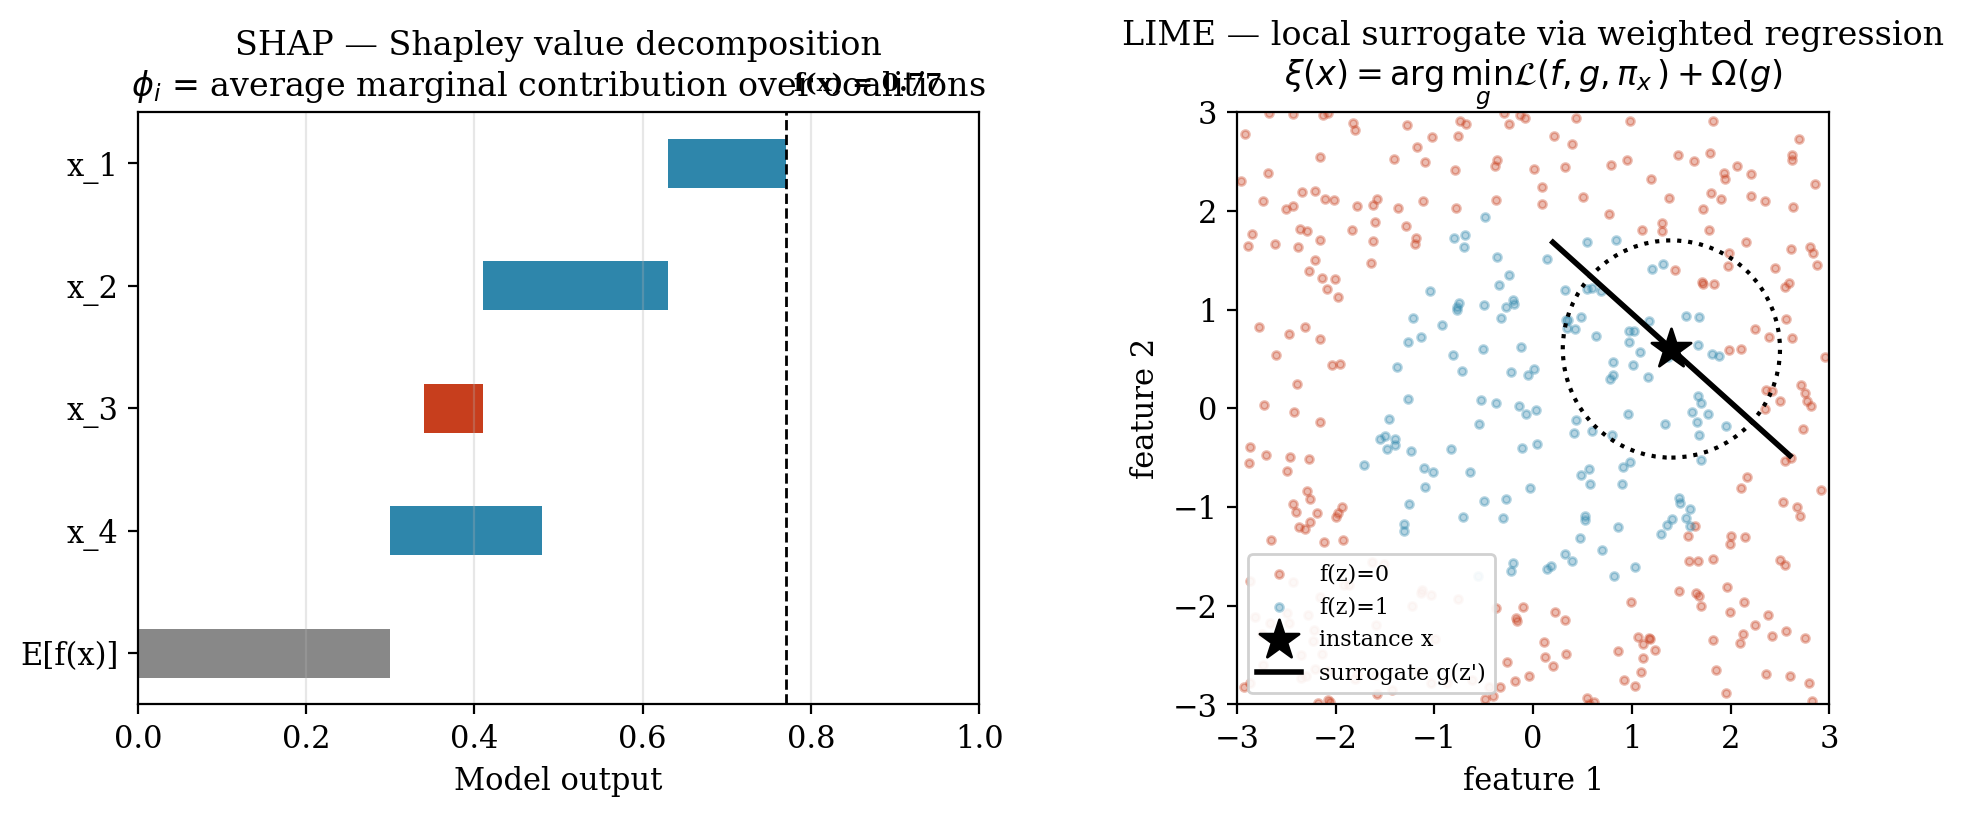
\includegraphics[width=0.95\textwidth]{sparsity_fig_2_1_shap_vs_lime.png}
    \caption{Mechanistic comparison of SHAP and LIME. SHAP (left) decomposes the
    model output $f(x)$ as the sum of the expected output $E[f(x)]$ and the
    per-feature Shapley contributions $\phi_i$; LIME (right) fits a locally
    weighted linear surrogate $g$ to perturbed samples drawn around the instance
    $x$ within the locality kernel $\pi_x$.}
    \label{fig:shap_vs_lime}
\end{figure}

\subsection{Multi-Tenant Architecture and Data Isolation}
\label{subsec:multi-tenant}

A \emph{multi-tenant} application is one in which a single deployment of the
software serves multiple independent customer organizations, called
\emph{tenants}, while preserving the logical isolation of each tenant's data,
configuration and access permissions~\citep{bezemer2010multi}. The literature
recognizes three canonical isolation models, in order of increasing isolation
strength: (i) \emph{shared schema} with a discriminator column,
(ii) \emph{schema-per-tenant} within a single database, and
(iii) \emph{database-per-tenant}, in which each tenant is allocated a
physically distinct database~\citep{krebs2014multitenancy}.

The system studied in this thesis adopts the database-per-tenant model on
PostgreSQL, orchestrated by Django~4.2 via a routed connection layer that
resolves each inbound request to the appropriate tenant database. This choice
maximizes data-isolation guarantees: a SQL injection or query-construction
error in one tenant's context cannot, by construction, leak rows belonging to
another tenant. From a security and compliance perspective the model is
conservative and defensible.

From a machine-learning perspective, however, the same isolation property has
a corrosive side effect. Each tenant's ML pipeline is confined to that
tenant's own database, which means that the training corpus available to any
per-tenant model is bounded above by the operational history of a single SME.
A tenant who joined the platform three weeks ago and has issued forty invoices
simply has no way to participate in a training process that requires thousands
of labelled observations. The isolation that protects the SME tenant's data
from its competitors also \emph{starves} the ML and XAI subsystems that the
platform offers to that same SME. This structural tension between
data-isolation security and data-volume sufficiency is the architectural
origin of the cold-start regime addressed by this thesis.

\subsection{The Cold-Start Problem in ML versus XAI}
\label{subsec:cold-start}

The traditional cold-start problem, as formulated in the recommender-systems
and personalization literature, is \emph{predictive}: a newly-introduced user
or item lacks the interaction history required for an accurate prediction to
be made. The remedies developed in that literature---content-based fallbacks,
transfer learning, meta-learning and warm-start priors---are correspondingly
aimed at improving the \emph{prediction}.

The present thesis introduces a conceptually distinct second variant, the
\emph{explanatory} cold-start. An explanatory cold-start occurs when the
system possesses enough engineering machinery to \emph{emit} a prediction and
an accompanying SHAP or LIME explanation, but the underlying model is too
poorly fit to make either the prediction \emph{or} the explanation faithful
representations of any real-world phenomenon. Critically, the failure modes of
predictive and explanatory cold-start are not aligned: a predictive cold-start
fails \emph{loudly} (the prediction is wrong and is sometimes recognized as
such), whereas an explanatory cold-start fails \emph{silently and confidently}
(a polished, axiomatically-grounded SHAP attribution is rendered for a model
that has collapsed to chance performance).

This silent failure mode is what this thesis names the \textbf{hallucinated
explanation}: an explanation that is \emph{internally} faithful (to the
degenerate model that produced it) and \emph{externally} meaningless (with
respect to the business process the model was intended to capture). The
phenomenon is not a flaw of SHAP or LIME \emph{per se}---both methods are
operating exactly as specified---but rather a failure of the surrounding
system to recognize that \emph{explaining a noise-fitting model is a category
error}. The architectural implication is that no defensible XAI deployment in
a multi-tenant SaaS context can treat the explanation layer as unconditional;
it must be guarded by a mechanism that detects the explanatory cold-start
regime and refuses to enter it.

\subsection{Metrics for Explanation Reliability}
\label{subsec:metrics}

To convert the abstract notion of ``explanation reliability'' into a
measurable quantity, this thesis adopts and combines several established
metrics from the XAI-stability literature.

\paragraph{Spearman Rank Correlation ($\rho$).}
Given two rankings of $n$ features---one produced by the explainer under
evaluation and one produced by a reference \emph{data-rich baseline} explainer
trained on the largest available data partition---the Spearman rank
correlation is defined as
\begin{equation}
\rho \;=\; 1 \;-\; \frac{6 \sum_{i=1}^{n} d_i^{\,2}}{n\,(n^2 - 1)},
\label{eq:spearman}
\end{equation}
where $d_i$ is the difference between the ranks of feature $i$ under the two
rankings. A value of $\rho = 1$ denotes perfect rank agreement (the
sparse-tenant model orders feature importances identically to the data-rich
baseline); a value of $\rho \le 0$ denotes that the two rankings are
uncorrelated or reversed. A conventional threshold of $\rho \ge 0.70$ is used
in the explanation-stability literature as the lower bound of operationally
defensible ranking agreement; below this value, the explainer can no longer
be regarded as recovering the same feature-importance signal as a
well-trained reference.

\paragraph{SHAP Absolute Variance.}
Defined as the variance of the per-feature mean absolute SHAP value across the
feature set, this metric quantifies \emph{how concentrated} the explanation
mass is on a small number of features versus how \emph{evenly distributed} it
is across many. A high SHAP absolute variance indicates that a single feature
is dominating the attribution---a signature symptom of over-fitting to a
spurious correlation in a small sample. A low variance indicates that
explanatory weight is distributed across a plausible coalition of features,
consistent with a well-regularized model. In the experimental results of this
thesis, SHAP absolute variance rises from $0.0224$ at the data-rich tier
($n = 50{,}000$) to $0.2017$ at the $n = 200$ tier, a nearly nine-fold spike
that empirically witnesses the over-fitting collapse of the sparse-tenant
model.

Complementary metrics employed in the empirical study include SHAP entropy
(an information-theoretic measure of the diffuseness of the attribution
distribution), the top-$k$ Jaccard similarity of LIME feature selections
across repeated runs (a measure of explanation \emph{stability}), and
standard predictive metrics such as AUC-ROC. The full operational definitions
are deferred to Chapter~\ref{ch:methodology}; what matters for the theoretical
framework is that, taken together, these metrics make it possible to
\emph{measure}, rather than merely assert, the degradation of explanation
reliability as a continuous function of tenant data volume.

\begin{figure}[h]
    \centering
    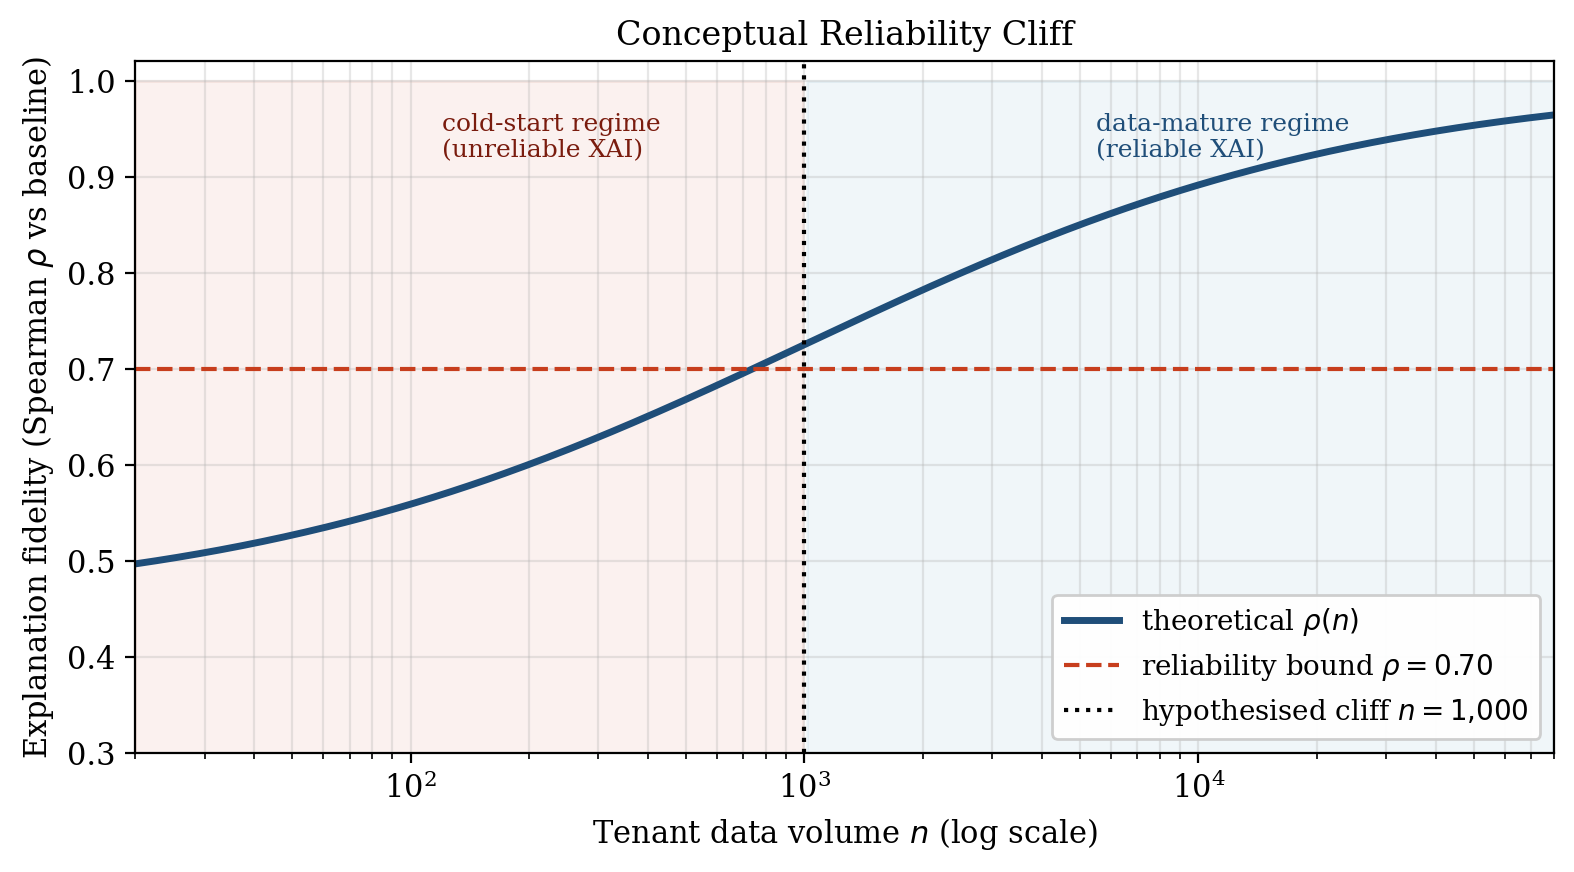
\includegraphics[width=0.85\textwidth]{sparsity_fig_2_2_reliability_cliff_theory.png}
    \caption{Conceptual \emph{Reliability Cliff} relating tenant data volume
    $n$ (log scale) to explanation fidelity (Spearman $\rho$ against the
    data-rich baseline). The horizontal dashed line marks the $\rho = 0.70$
    reliability bound; the vertical dotted line marks the hypothesised
    cold-start threshold at $n = 1{,}000$.}
    \label{fig:reliability_cliff_theory}
\end{figure}

\section{Research Thinking Framework}
\label{sec:lit-framework}

The conceptual architecture of this research connects the theoretical
components reviewed above into a single causal chain, which simultaneously
functions as the logical scaffold of the empirical study and as the blueprint
for the proposed architectural solution.

The chain begins with \textbf{multi-tenant data isolation}. The
database-per-tenant architecture adopted by the studied ERP enforces strict
logical and physical separation between tenant datasets. This isolation is
non-negotiable from a security and regulatory standpoint, yet it has the
unavoidable consequence that the data available to each tenant's ML pipeline
is bounded by that tenant's own operational history. For mature tenants this
bound is large; for cold-start SMEs it is small, sometimes vanishingly so.

This produces the second link in the chain: \textbf{data sparsity} at the
tenant level. Sparsity is not a transient anomaly but a \emph{structural}
property of the multi-tenant SaaS distribution, in which a long tail of small
tenants persists indefinitely alongside a smaller head of data-rich
enterprises.

Sparsity then propagates into the ML layer, where per-tenant models trained
on small samples regress toward random performance. Under classical ML
evaluation this is recognized as the predictive cold-start. However, in any
deployment in which SHAP or LIME is applied unconditionally to such a
degraded model, the sparsity propagates one layer further into the XAI
subsystem, producing the third link in the chain: \textbf{XAI degradation in
the form of hallucinated explanations}---confident, well-formatted
attributions over a model that has no genuine signal to attribute.

The fourth link is \textbf{empirical measurement}. Hallucinated explanations
are dangerous precisely because they do not announce themselves. The
framework therefore prescribes that the phenomenon be made visible through
quantitative metrics: Spearman rank correlation against a data-rich baseline
(fidelity), absolute SHAP variance and SHAP entropy (stability), and LIME
top-$k$ Jaccard similarity (overlap). The empirical layer of the framework
operationalizes the conceptual claim that the failure of XAI under sparsity
is not merely \emph{theoretically plausible} but \emph{empirically
measurable} and, therefore, \emph{engineering-actionable}.

The chain closes with the fifth link: \textbf{the architectural solution}.
Because the failure regime can be detected ahead of time from a single
observable property of the tenant---its row count---the framework proposes
the \textbf{Maturity-Aware AI Routing} pattern. Tenants whose data volume
falls below the empirically-identified cold-start threshold ($n \le 1{,}000$,
as established in Chapter~\ref{ch:results}) are routed to a global,
heuristic-based explanation strategy derived from the data-rich baseline;
tenants at or above the threshold receive local SHAP/LIME explanations. The
routing decision is made at the architectural layer, before any explanation
is generated, and is therefore guaranteed to prevent the rendering of a
hallucinated explanation regardless of downstream UI behaviour.

\begin{figure}[h]
    \centering
    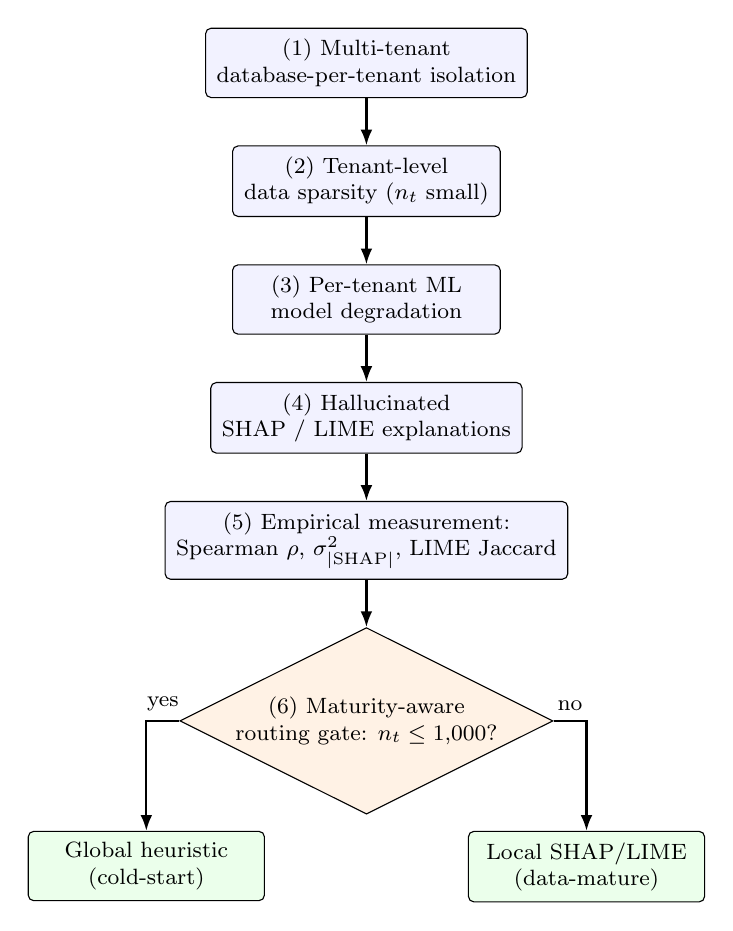
\begin{tikzpicture}[
        node distance=6mm and 8mm,
        every node/.style={font=\footnotesize},
        box/.style={draw,rounded corners=2pt,align=center,inner sep=4pt,
                    minimum width=3.4cm,minimum height=8mm,fill=blue!5},
        decision/.style={draw,diamond,aspect=2,align=center,inner sep=1pt,
                         minimum width=3.4cm,fill=orange!10},
        outcome/.style={draw,rounded corners=2pt,align=center,inner sep=4pt,
                        minimum width=3.0cm,minimum height=8mm,fill=green!8},
        arr/.style={-{Latex[length=2mm]},thick},
    ]
        \node[box] (n1) {(1) Multi-tenant\\database-per-tenant isolation};
        \node[box,below=of n1] (n2) {(2) Tenant-level\\data sparsity ($n_t$ small)};
        \node[box,below=of n2] (n3) {(3) Per-tenant ML\\model degradation};
        \node[box,below=of n3] (n4) {(4) Hallucinated\\SHAP / LIME explanations};
        \node[box,below=of n4] (n5) {(5) Empirical measurement:\\Spearman $\rho$, $\sigma^2_{|\text{SHAP}|}$, LIME Jaccard};
        \node[decision,below=of n5] (gate) {(6) Maturity-aware\\routing gate: $n_t \le 1{,}000$?};
        \node[outcome,below left=8mm and 1mm of gate] (heur) {Global heuristic\\(cold-start)};
        \node[outcome,below right=8mm and 1mm of gate] (local) {Local SHAP/LIME\\(data-mature)};
        \draw[arr] (n1) -- (n2);
        \draw[arr] (n2) -- (n3);
        \draw[arr] (n3) -- (n4);
        \draw[arr] (n4) -- (n5);
        \draw[arr] (n5) -- (gate);
        \draw[arr] (gate.west) -| node[above,pos=0.25] {yes} (heur.north);
        \draw[arr] (gate.east) -| node[above,pos=0.25] {no}  (local.north);
    \end{tikzpicture}
    \caption{Research conceptual framework: from multi-tenant isolation to the
    Maturity-Aware AI Routing decision gate. The cold-start branch is taken
    inclusively at $n_t \le 1{,}000$ (equivalently, the code-side guard
    $n_t < \textsf{MIN\_LOCAL\_EXPLANATION\_RECORDS}$ with the constant set
    to $1{,}001$).}
    \label{fig:research_framework}
\end{figure}

The framework is deliberately constructed so that each conceptual link is, in
the chapters that follow, either operationalized as a methodological
procedure (Chapter~\ref{ch:methodology}), instantiated as an experimental
artefact (Chapter~\ref{ch:results}), or implemented as a software component
within that same chapter's reference implementation. The theoretical crux
that the framework formalizes---and that the remainder of the thesis
empirically defends---is the strict separation between \emph{predictive
accuracy} and \emph{explanatory fidelity}, and the architectural consequence
that, in multi-tenant SaaS ERPs, the latter requires its own dedicated
reliability gate.

% !TEX root = ../sparsity_thesis.tex
\chapter{Research Methodology}
\label{ch:methodology}

This chapter describes the methodology by which the research questions
formulated in Chapter~\ref{ch:introduction} were operationalised into a
reproducible empirical study. The chapter follows the canonical
CRISP-DM-aligned sequence of \emph{problem scoping}, \emph{data gathering},
\emph{data preparation}, \emph{modelling}, \emph{evaluation}, and
\emph{deployment}, adapted to the specific concerns of measuring explanation
fidelity rather than predictive accuracy alone.

\section{Problem Scoping}
\label{sec:problem-scoping}

\subsection{Research Objectives}
\label{subsec:meth-objectives}

In direct continuation of Chapter~\ref{ch:introduction}, this research pursues
four objectives, which together translate the abstract research questions
(RQ1--RQ3) into actionable engineering targets:

\begin{enumerate}
    \item \textbf{Quantify XAI degradation under data sparsity.} Establish,
    through controlled cross-sectional experimentation, the empirical
    relationship between tenant-level training-data volume and the fidelity
    and stability of post-hoc SHAP and LIME explanations.
    \item \textbf{Identify the cold-start XAI threshold.} Determine the
    data-volume boundary at which local post-hoc explanations cease to be
    operationally reliable, characterising the non-linear \emph{Reliability
    Cliff} hypothesised in Chapter~\ref{ch:literature-review}.
    \item \textbf{Design the Maturity-Aware AI Routing architecture.} Specify
    a tenant-aware tier-logic gate that conditions the choice of explanation
    strategy on each tenant's data maturity.
    \item \textbf{Implement and evaluate the tier-logic gate.} Realise the
    proposed pattern as a concrete software component inside the studied
    Django / PostgreSQL ERP, and verify that it routes correctly and preserves
    backward compatibility.
\end{enumerate}

\subsection{Research Scope}
\label{subsec:meth-scope}

The methodological scope of this study was constrained as follows in order to
preserve interpretability and reproducibility:

\begin{itemize}
    \item \textbf{Platform.} A single multi-tenant ERP system based on
    Django~4.2 and PostgreSQL, configured under the database-per-tenant
    isolation model.
    \item \textbf{Prediction tasks.} Three ERP-native supervised tabular
    classification problems: Late Delivery Risk prediction, Lead Scoring, and
    Employee Attrition.
    \item \textbf{XAI techniques.} Two post-hoc, model-agnostic explainers
    were evaluated: SHAP (specifically the \emph{TreeExplainer} and
    \emph{LinearExplainer} variants) and LIME (in its tabular form).
    Intrinsically interpretable models and gradient-based explainers for deep
    networks were not within scope.
    \item \textbf{Evaluation mode.} Offline, cross-sectional simulation
    against curated open-source datasets. No live SaaS tenant traffic was
    used, and no longitudinal observation of data accumulation over real
    calendar time was performed.
    \item \textbf{Architectural pattern.} Only the Maturity-Aware AI Routing
    pattern was implemented and evaluated; alternative remedies for sparsity
    (transfer learning, federated learning, meta-learning) were noted but
    deferred to future work.
\end{itemize}

\subsection{Research Contribution}
\label{subsec:meth-contribution}

Two distinct but interdependent contributions emerge from this methodology:

\begin{enumerate}
    \item \textbf{An empirical contribution.} The study quantifies, for the
    first time in a B2B multi-tenant ERP setting, the degradation of post-hoc
    explanation fidelity as a continuous function of tenant data volume,
    using a coherent panel of metrics (Spearman rank correlation, SHAP
    absolute variance, SHAP entropy, LIME top-$k$ Jaccard similarity). The
    resulting curves localise the \emph{Reliability Cliff} and produce a
    defensible numerical threshold for the cold-start regime.
    \item \textbf{An architectural contribution.} The study delivers the
    \textbf{Maturity-Aware AI Routing} pattern as a concrete, implementable
    software-engineering artefact, instantiated inside a real Django ERP
    codebase. The contribution is not merely conceptual: it includes the
    routing rule, its empirically-derived threshold, the global-heuristic
    fallback artefact, and the integration discipline by which the gate is
    added without disturbing the existing ML production code path.
\end{enumerate}

\section{Data Gathering}
\label{sec:data-gathering}

\subsection{Open-Source ERP Datasets}
\label{subsec:datasets}

In the absence of an ethically- and legally-shareable real multi-tenant SaaS
dataset, two well-established open-source corpora were adopted as proxies for
ERP operational data. Both datasets were selected for their structural
similarity to the kinds of tabular, time-stamped, business-process records
that an ERP routinely accumulates.

\paragraph{Olist Brazilian E-Commerce Public Dataset.}
This corpus, released by the Brazilian marketplace platform Olist and hosted
on Kaggle, comprises approximately $100{,}000$ orders placed between 2016 and
2018, distributed across nine relational tables covering customers, sellers,
orders, order items, payments, reviews, and products. After joining the
order, payment, and item tables on the canonical \texttt{order\_id} key, the
resulting unified table contained $N = 96{,}460$ rows. This corpus was used
as the empirical substrate for the \textbf{Late Delivery Risk} prediction
task, operationalised as the binary event ``actual delivery date later than
the estimated delivery date'' (formally,
$\mathbf{1}[\textit{order\_delivered\_customer\_date} >
\textit{order\_estimated\_delivery\_date}]$). The Olist corpus exposes
delivery-time observables but not invoice payment-time observables, so the
literal target is delivery lateness rather than payment lateness; for the
purposes of this study the construct of interest is the wider class of
\emph{ERP-style operational-risk prediction} (sparse, tabular, time-stamped
business-process records with a small positive-class prevalence), of which
late delivery is one instance and late payment is another. The proposed
architectural pattern (Section~\ref{subsec:routing-arch}) is task-agnostic and
generalises directly to the late-payment prediction service
(\texttt{LatePaymentPredictor}) of the studied ERP, which shares the same
tabular, sparsity-conditioned structure.

\paragraph{Synthetic CRM Leads Corpus.}
\label{para:crm-leads-synth}
No public CRM lead-scoring dataset of sufficient size and structural realism
was identified during corpus selection, and the studied ERP's own production
CRM tables could not be released for academic reuse. To enable the
cross-task replication while preserving the methodological invariants of
the Late Delivery Risk experiment (tabular structure, stratified sparsity
gradient, deterministic train/test partitions), a \emph{synthetic CRM
Leads corpus} was generated and stored at
\texttt{datasets/crm\_leads\_dataset.csv}. The corpus contains $N = 5{,}000$
lead records (one row per lead) with $20$ raw columns; after dropping
personally-identifying and post-event fields and one-hot encoding the
categorical attributes \texttt{source}, \texttt{service\_interest},
\texttt{country}, and \texttt{job\_title}, the model-facing feature matrix
comprises $34$ covariates. The binary target is
$\textsf{won} = \mathbf{1}[\textit{status} = \text{\textsf{won}}]$, with a
class prevalence of $21.3\%$ positives.

The four numeric predictors are \texttt{estimated\_value} (deal size),
\texttt{probability} (sales-team-assigned win likelihood at the time of
scoring), \texttt{activity\_count} (count of touchpoints recorded against
the lead), and \texttt{days\_in\_pipeline} (age of the lead since
\texttt{created\_at}). The four categorical predictors are
\texttt{source}, \texttt{service\_interest}, \texttt{country}, and
\texttt{job\_title}.

Three leakage controls are imposed by construction. First, the column
\texttt{conversion\_date} is populated \emph{only} for converted leads and
is therefore a post-event variable that perfectly determines the target;
it is dropped before training. Second, the raw \texttt{status} column is
the target itself and is excluded from features. Third, all
identifier and PII columns (\texttt{lead\_number},
\texttt{first\_name}, \texttt{last\_name}, \texttt{email},
\texttt{phone}, \texttt{mobile}, \texttt{company\_name}, \texttt{city},
\texttt{created\_at}, \texttt{last\_contact\_date}) carry no
predictive content under the chosen feature representation and are
dropped. The resulting feature matrix therefore represents the current
snapshot of a lead at the moment a scoring call would be issued, mirroring
how CRM systems expose lead state to a downstream model in production.

The rationale for using a synthetic corpus is twofold: (i)~it permits full
release of the dataset alongside the simulator script
(\texttt{thesis/scripts/lead\_scoring\_simulator.py}), ensuring exact
reproducibility of the cross-task replication, and (ii)~it allows the same
stratified slicing procedure to be applied with controlled class prevalence
and controlled feature semantics, isolating the sparsity treatment from
confounding distributional drift. The principal limitation is one of
external validity: because the records are drawn from a parametric
generator rather than a real CRM workflow, the absolute level of
predictive performance and the specific feature importances reported in
Chapter~\ref{ch:results} should be read as illustrative of \emph{the
shape of the sparsity-induced degradation curve}, not as point estimates
transferable to any particular commercial CRM deployment. The structural
findings of interest---the monotone collapse of rank agreement, the
order-of-magnitude expansion of attribution variance, and the cold-start
flip of predictive performance---are nevertheless replicated on this
corpus and are interpreted as evidence of the architectural pattern
rather than as production-grade performance estimates.

\paragraph{IBM HR Analytics Employee Attrition Dataset.}
This corpus, released by IBM Watson Analytics, contains $1{,}470$ employee
records labelled with a binary \texttt{Attrition} outcome and 34 covariates
spanning demographic, compensation, tenure, and performance-rating fields. It
was adopted as the empirical substrate for the \textbf{Employee Attrition}
prediction task, which directly corresponds to the HR-attrition use case
inside the ERP's HR module.

The suitability of these datasets as ERP proxies rests on three structural
correspondences: (i)~both are tabular, transactionally-keyed records of
business events; (ii)~both expose covariates whose semantics (timestamps,
monetary amounts, tenure, categorical statuses) match those of typical ERP
fields; and (iii)~the volume of each corpus is large enough to support the
construction of a five-tier sparsity gradient while leaving a held-out
evaluation partition intact.

\section{Data Preparation}
\label{sec:data-prep}

\subsection{Feature Engineering}
\label{subsec:feature-eng}

Each raw record was passed through a deterministic feature-engineering
pipeline that produced 13 engineered covariates per row, grouped into four
families:

\begin{itemize}
    \item \textbf{Temporal-derivative features.} From the raw
    \texttt{order\_purchase\_timestamp},
    \texttt{order\_approved\_at}, and
    \texttt{order\_estimated\_delivery\_date} columns, the variables
    \texttt{approval\_delay\_hours} (purchase-to-approval interval),
    \texttt{estimated\_delivery\_days} (the courier ETA quoted to the
    customer at order time),
    \texttt{purchase\_hour}, and \texttt{purchase\_dow} (day-of-week of
    purchase) were computed.
    \item \textbf{Monetary features.} From the order-items and payments
    tables, the variables \texttt{payment\_value}, \texttt{freight\_value},
    and \texttt{price\_total} (aggregate line-item total per order) were
    derived.
    \item \textbf{Cardinality features.} The variables \texttt{num\_items}
    (line-item count) and \texttt{payment\_installments} (number of
    instalments selected at checkout) were extracted, capturing order-level
    structural complexity.
    \item \textbf{Categorical encodings.} The \texttt{payment\_type} field
    was one-hot encoded into four indicator columns
    (\texttt{credit\_card}, \texttt{boleto}, \texttt{voucher},
    \texttt{debit\_card}).
\end{itemize}

\paragraph{Leakage-avoidance constraint.}
\label{para:leakage-avoidance}
All engineered covariates listed above are restricted, by construction, to
information that would be available at the moment a late-payment prediction
is required---namely, at order approval / invoice issuance. Timestamps from
the delivery pipeline---\texttt{order\_delivered\_carrier\_date} and
\texttt{order\_delivered\_customer\_date}---are reserved \emph{solely} for
the construction of the binary target and are explicitly excluded from the
feature matrix. In particular, an earlier version of this study included
the covariate \texttt{carrier\_delay\_hours}, defined as the interval
between \texttt{order\_approved\_at} and
\texttt{order\_delivered\_carrier\_date}; it was subsequently removed
because, although it precedes the customer-delivery event, it is itself a
delivery-pipeline observable and is therefore not realised at prediction
time in a deployed ERP late-payment workflow. Its inclusion would have
constituted a textbook instance of target leakage and would have inflated
the predictive metrics reported in Chapter~\ref{ch:results} without
reflecting a capability the model would possess in production. The
restriction reduces the engineered feature count from $14$ to $13$ and
rules out the trivial metric inflation that would otherwise arise from
explaining a delivery-time outcome with a delivery-time covariate.

Missing values were imputed using the column-wise median for numeric
features and the modal value for categorical features, and the resulting
matrix was standardised by z-scoring of numeric columns. The binary target
\texttt{is\_late} was constructed as
$\mathbf{1}[\textit{order\_delivered\_customer\_date} >
\textit{order\_estimated\_delivery\_date}]$. The overall positive-class
prevalence after joining was $8.1\%$, establishing a moderately imbalanced
classification problem consistent with typical ERP late-delivery (and, by structural analogy, late-payment) base rates.

\subsection{Multi-Tenant Simulation Strategy}
\label{subsec:multi-tenant-sim}

Because no commercially-shareable multi-tenant ERP dataset exists at the
scale required to expose a sparsity gradient, this study adopted a
\emph{stratified data-volume slicing} strategy to simulate the long-tail
distribution of tenant maturities observed empirically in production SaaS
platforms. The procedure was as follows:

\begin{enumerate}
    \item The unified, feature-engineered Olist late-delivery table
    ($N = 96{,}460$, positive prevalence $8.1\%$) was first partitioned into
    a global hold-out evaluation set ($20\%$, $n = 19{,}292$) using a
    stratified random split with seed $\textsf{SEED} = 42$, preserving the
    late-delivery class prevalence.
    \item From the remaining $77{,}168$ training rows, five disjoint
    \emph{simulated tenant partitions} were drawn by stratified random
    sampling without replacement, each preserving the global positive-class
    prevalence (Table~\ref{tab:tenant-tiers}).
    \item Each tenant partition was subsequently subjected to its own
    internal $80/20$ stratified train/validation split, again with
    $\textsf{SEED} = 42$, yielding tenant-local training and validation folds.
    \item All five tenants were evaluated against the \emph{shared} global
    hold-out evaluation set, so that cross-tenant comparisons of predictive
    performance and explanation fidelity referred to an identical test
    distribution and were therefore directly comparable.
\end{enumerate}

\begin{table}[h]
\centering
\caption{Simulated tenant tiers used in the sparsity experiment.}
\label{tab:tenant-tiers}
\renewcommand{\arraystretch}{1.2}
\begin{tabular}{@{}clrl@{}}
\toprule
\textbf{Tier} & \textbf{Tenant label} & \textbf{Sample size $n$} &
\textbf{Interpretation} \\
\midrule
A & Data-Rich    & 50{,}000 & Mature enterprise tenant \\
B & Medium       &  5{,}000 & Established SME tenant \\
C & Sparse       &  1{,}000 & Onboarded SME tenant \\
D & Very Sparse  &      200 & Newly-active SME tenant \\
E & Cold-Start   &       50 & Just-onboarded SME tenant \\
\bottomrule
\end{tabular}
\end{table}

This stratified slicing strategy is methodologically conservative: by
preserving the class prevalence at every tier, it ensures that any observed
degradation in predictive or explanatory quality at smaller $n$ is
attributable to \emph{data volume}, not to changes in label distribution.
The same procedure was applied, with appropriate sample sizes, to the IBM HR
Attrition corpus.

\begin{figure}[h]
    \centering
    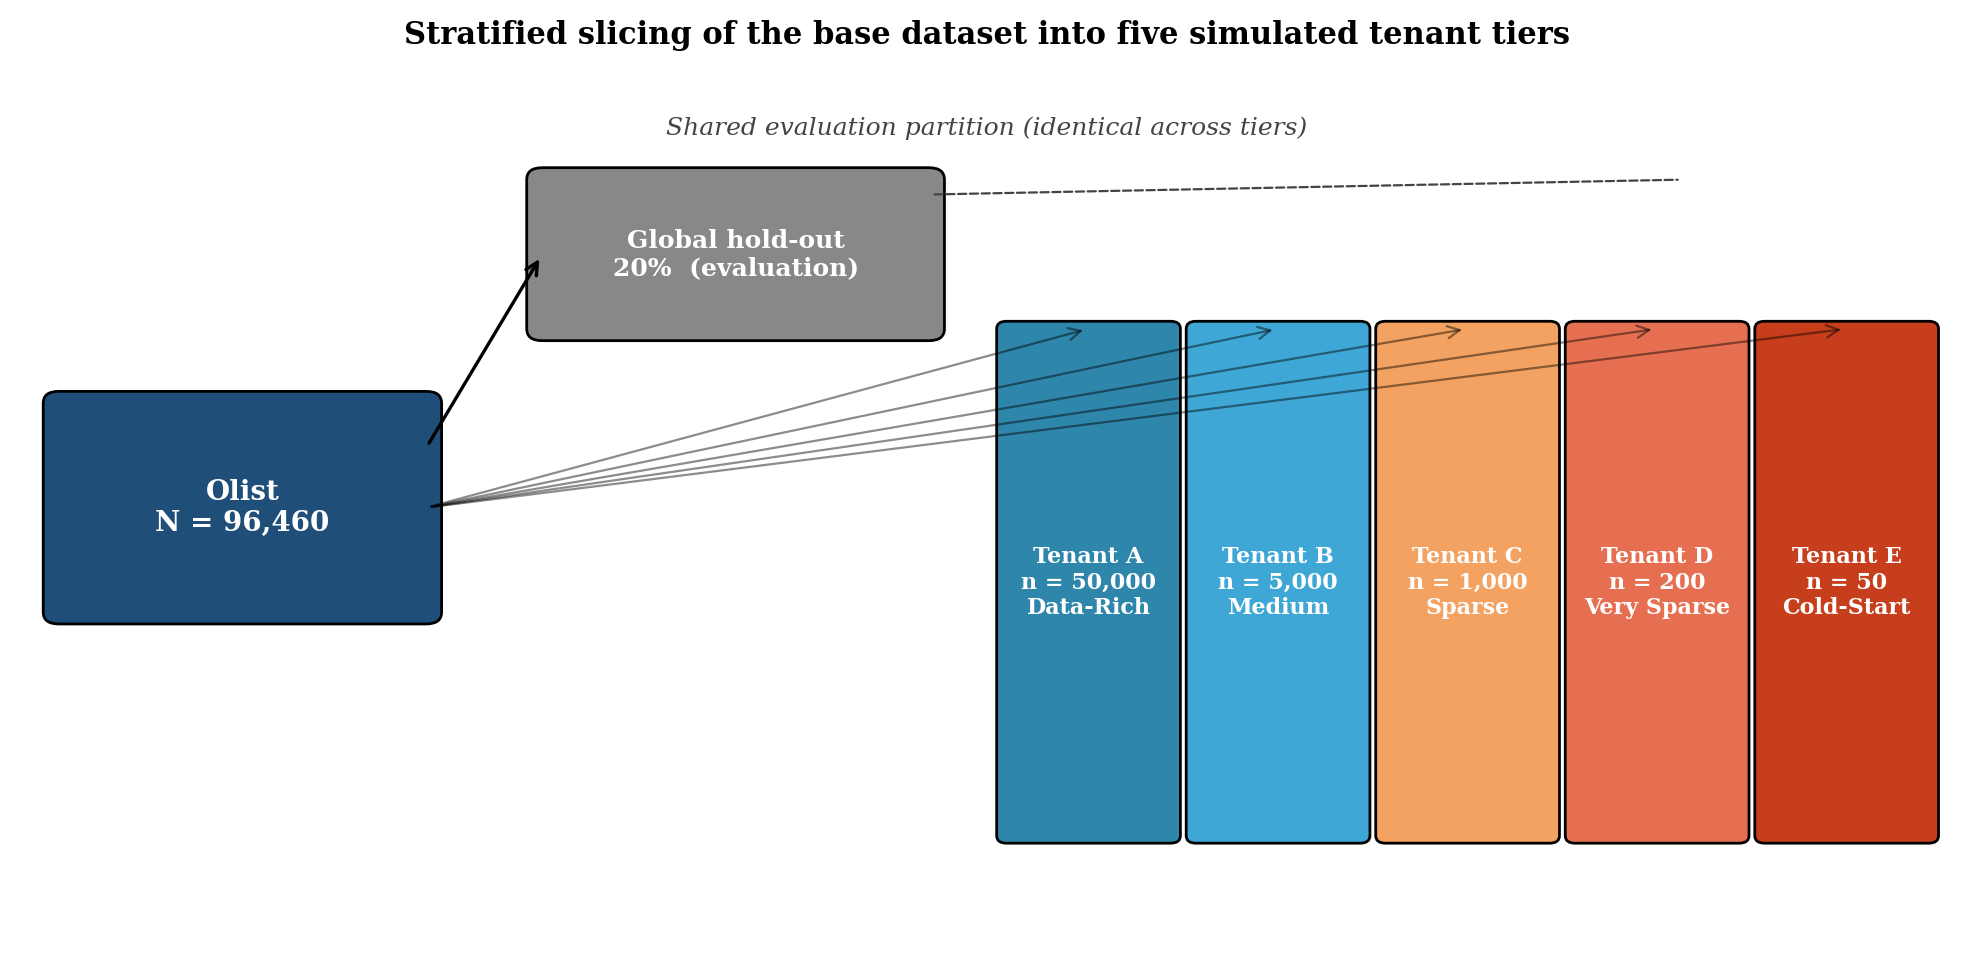
\includegraphics[width=0.95\textwidth]{sparsity_fig_3_1_simulation_strategy.png}
    \caption{Stratified slicing of the base Olist dataset ($N = 96{,}460$)
    into a shared $20\%$ global hold-out evaluation partition and five
    disjoint simulated tenant tiers ($n = 50{,}000$; $5{,}000$; $1{,}000$;
    $200$; $50$), with class prevalence preserved at each tier.}
    \label{fig:sim-strategy}
\end{figure}

\section{Modelling}
\label{sec:modelling}

\subsection{Machine Learning Algorithms}
\label{subsec:algorithms}

Three supervised classifiers were selected, each appropriate to one
prediction task and each representative of a different model family widely
used in operational ERP analytics:

\begin{itemize}
    \item \textbf{Late Delivery Risk --- Gradient Boosting Machine (GBM).}
    Implemented via scikit-learn's \texttt{GradientBoostingClassifier} with
    $n_{\text{estimators}} = 100$, $\textit{max\_depth} = 3$,
    $\textit{learning\_rate} = 0.1$, and the default deviance loss. GBMs were
    selected because tree-ensemble methods are the de facto industry
    standard for tabular financial classification, and because their
    structure is directly compatible with SHAP's polynomial-time
    \emph{TreeExplainer}.
    \item \textbf{Lead Scoring --- Gradient Boosting Machine (GBM).}
    Implemented via scikit-learn's \texttt{GradientBoostingClassifier} with
    $n_{\text{estimators}} = 200$, $\textit{max\_depth} = 3$,
    $\textit{learning\_rate} = 0.05$, and the default deviance loss. The
    same algorithmic family as the Late Delivery Risk task was retained
    deliberately, so that any cross-task differences in the sparsity-induced
    degradation trajectory can be attributed to substrate properties
    (dimensionality, feature dominance, class prevalence) rather than to
    algorithmic confounders. An earlier design used Logistic Regression as a
    representative linear baseline; it was superseded by the GBM variant
    once the replication scope was extended, in order to keep the algorithmic
    surface invariant across tasks and thereby strengthen the
    architectural-pattern claim.
    \item \textbf{Employee Attrition --- Random Forest.} Implemented via
    scikit-learn's \texttt{RandomForestClassifier} with $n_{\text{estimators}}
    = 200$, $\textit{max\_depth} = \text{None}$,
    \texttt{class\_weight = "balanced"}, and \texttt{random\_state = 42}.
    Random forests were chosen for their robustness on small-to-medium
    tabular HR datasets, where the IBM corpus is itself only $1{,}470$ rows.
\end{itemize}

For each prediction task, an identical algorithm was retrained from scratch
on each of the five tenant partitions, producing five independent fitted
models per task. All randomness was controlled via $\textsf{SEED} = 42$ to
guarantee bit-level reproducibility.

\subsection{Explainable AI (XAI) Integration}
\label{subsec:xai-integration}

After fitting, each per-tenant model was subjected to a uniform post-hoc XAI
pipeline:

\begin{itemize}
    \item \textbf{SHAP attribution.} For the tree-based models
    (GBM, Random Forest), SHAP values were computed via the polynomial-time
    \texttt{shap.TreeExplainer}, yielding both per-instance attribution
    vectors and the global mean-absolute-SHAP feature-importance ranking.
    For the Logistic Regression model, \texttt{shap.LinearExplainer} was
    used with the matching background distribution.
    \item \textbf{LIME surrogate explanation.} For every model, local
    explanations were generated using
    \texttt{lime.lime\_tabular.LimeTabularExplainer} configured with
    \texttt{mode="classification"}, $5{,}000$ perturbation samples per
    explanation, and a Gaussian kernel width of $\sqrt{M}$ where $M$ is the
    number of features. The top-$5$ features per instance were retained for
    downstream stability analysis.
    \item \textbf{Sampling for evaluation.} Because LIME is stochastic,
    every LIME-based metric was averaged over $50$ independent runs per
    instance, and SHAP values were always computed on the full shared global
    hold-out set so that cross-tenant comparisons referred to identical
    inputs.
\end{itemize}

This pipeline yields, for each (task, tenant) combination, a paired bundle
consisting of the trained model, the global SHAP feature-importance ranking,
the per-instance SHAP attributions on the hold-out set, and the LIME top-$5$
selections together with their stability statistics.

\subsection{Maturity-Aware AI Routing Architecture}
\label{subsec:routing-arch}

The architectural contribution of the methodology is the
\textbf{Maturity-Aware AI Routing} gate, which conditions the choice of
explanation strategy on the data maturity of the requesting tenant. The
gate was designed around three engineering principles: it must be
\emph{empirically grounded} (its threshold must be derived from the same
experiments that motivate its existence); it must be \emph{architecturally
minimal} (it must not require any change to the existing ML services); and
it must be \emph{fail-safe} (an unavailable global heuristic must not block
predictions).

The routing rule was formalised as follows. Let $n_t$ denote the number of
historically-recorded operational records for tenant $t$ (in the Late
Delivery Risk case, the count of invoices with status in $\{\textit{paid},
\textit{overdue}, \textit{partial}\}$), and let $\tau$ denote the
empirically-derived cold-start threshold. The architectural gate is then:
\begin{equation}
\textsf{explain}(t, x) \;=\;
\begin{cases}
    \textsf{GlobalHeuristic}() & \text{if } n_t \le \tau, \\
    \textsf{LocalShapLime}(t, x) & \text{otherwise.}
\end{cases}
\label{eq:routing}
\end{equation}

The boundary is deliberately \emph{inclusive} on the cold-start side: a
tenant with exactly $n_t = \tau$ records is routed to the global heuristic
rather than to a local explanation. This reflects the empirical finding
(Section~\ref{subsec:threshold}) that Tenant~C ($n = 1{,}000$) already lies
below the $\rho = 0.70$ reliability bound and already exhibits an inflated
SHAP variance, and it removes a latent off-by-one ambiguity in the
route-decision logic. The equivalent code-side formulation
$n_t < \textsf{MIN\_LOCAL\_EXPLANATION\_RECORDS}$ with
$\textsf{MIN\_LOCAL\_EXPLANATION\_RECORDS} = \tau + 1 = 1{,}001$ is
logically interchangeable and may be preferred where a strictly-less-than
guard is idiomatic.

The threshold $\tau$ was not chosen arbitrarily; as detailed in
Section~\ref{subsec:threshold} below, it was identified as $\tau = 1{,}000$
from the empirical fidelity curves derived in the modelling phase. The
threshold was encapsulated in the implementation as a class-level constant
\texttt{COLD\_START\_INVOICE\_THRESHOLD = 1000} (interpreted under the
inclusive boundary above) to allow operational re-tuning without code
change. The two branches of the gate correspond, in
the implementation, to:

\begin{itemize}
    \item \texttt{\_load\_global\_heuristic()} --- a memoised loader that
    reads the pre-computed cross-tenant SHAP feature-importance artefact
    (\texttt{cold\_start\_heuristic.json}, see
    Section~\ref{subsec:heuristic-artifact}) from disk and returns it as a
    structured explanation payload;
    \item \texttt{predict()} --- the existing per-tenant ML inference and
    SHAP/LIME explanation routine, left fully unchanged.
\end{itemize}

The gate itself is exposed as a new public method,
\texttt{predict\_or\_heuristic(invoice)}, which inspects
\texttt{\_invoice\_count()} and dispatches accordingly. The return payload
of both branches conforms to a single response schema (mode, threshold,
count, explanation), so that downstream consumers can be agnostic to which
branch was taken while still being able to surface the routing decision to
the end user.

\begin{figure}[h]
    \centering
    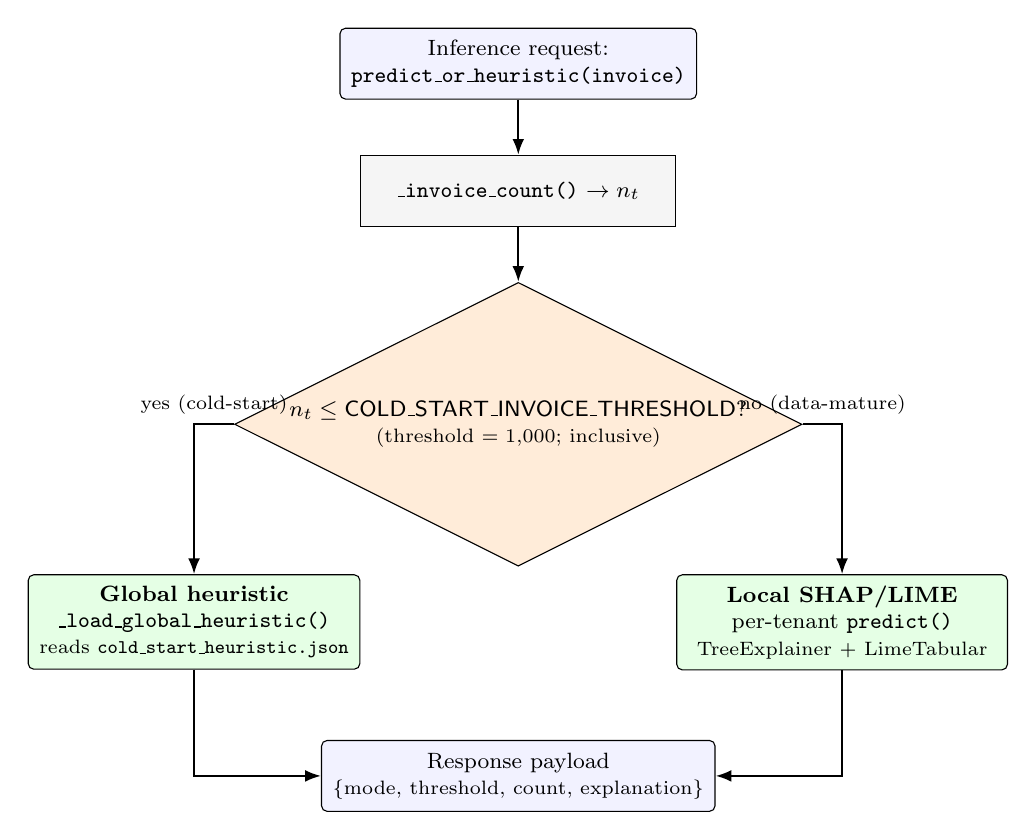
\begin{tikzpicture}[
        node distance=7mm and 10mm,
        every node/.style={font=\footnotesize},
        io/.style={draw,rounded corners=2pt,align=center,inner sep=4pt,
                   minimum width=3.6cm,minimum height=9mm,fill=blue!5},
        proc/.style={draw,align=center,inner sep=4pt,
                     minimum width=4.0cm,minimum height=9mm,fill=gray!8},
        decision/.style={draw,diamond,aspect=2,align=center,inner sep=1pt,
                         minimum width=4.2cm,fill=orange!15},
        outcome/.style={draw,rounded corners=2pt,align=center,inner sep=4pt,
                        minimum width=4.2cm,minimum height=10mm,fill=green!10},
        arr/.style={-{Latex[length=2mm]},thick},
    ]
        \node[io] (req) {Inference request:\\\texttt{predict\_or\_heuristic(invoice)}};
        \node[proc,below=of req] (count) {\texttt{\_invoice\_count()} $\rightarrow n_t$};
        \node[decision,below=of count] (gate) {$n_t \le \textsf{COLD\_START\_INVOICE\_THRESHOLD}$?\\\scriptsize (threshold $= 1{,}000$; inclusive)};
        \node[outcome,below left=10mm and 2mm of gate] (heur)
            {\textbf{Global heuristic}\\\texttt{\_load\_global\_heuristic()}\\\scriptsize reads \texttt{cold\_start\_heuristic.json}};
        \node[outcome,below right=10mm and 2mm of gate] (local)
            {\textbf{Local SHAP/LIME}\\per-tenant \texttt{predict()}\\\scriptsize TreeExplainer + LimeTabular};
        \node[io,below=22mm of gate] (resp) {Response payload\\\scriptsize\{mode, threshold, count, explanation\}};
        \draw[arr] (req) -- (count);
        \draw[arr] (count) -- (gate);
        \draw[arr] (gate.west) -| node[above,pos=0.25,font=\scriptsize] {yes (cold-start)} (heur.north);
        \draw[arr] (gate.east) -| node[above,pos=0.25,font=\scriptsize] {no (data-mature)} (local.north);
        \draw[arr] (heur.south) |- (resp.west);
        \draw[arr] (local.south) |- (resp.east);
    \end{tikzpicture}
    \caption{Maturity-Aware AI Routing architectural gate. The
    \texttt{LatePaymentPredictor.predict\_or\_heuristic()} method inspects the
    tenant's invoice count $n_t$ against the inclusive boundary
    $n_t \le \texttt{COLD\_START\_INVOICE\_THRESHOLD} = 1{,}000$
    (equivalently, $n_t < \textsf{MIN\_LOCAL\_EXPLANATION\_RECORDS} = 1{,}001$).
    Cold-start tenants are dispatched to the global heuristic served from
    \texttt{cold\_start\_heuristic.json}; data-mature tenants are dispatched
    to the per-tenant SHAP/LIME pipeline. Both branches emit a single
    schema-conformant response payload.}
    \label{fig:routing-arch}
\end{figure}

\section{Evaluation}
\label{sec:meth-evaluation}

\subsection{Predictive Performance Metrics}
\label{subsec:pred-metrics}

To establish a baseline against which the explanation-fidelity findings
could be interpreted, the standard panel of predictive metrics was computed
for each (task, tenant) combination on the shared global hold-out set:

\begin{itemize}
    \item \textbf{AUC-ROC} --- the area under the receiver-operating-
    characteristic curve, which is robust to class imbalance and serves as
    the primary headline metric of \emph{predictive} model quality.
    \item \textbf{F1-Score} --- the harmonic mean of precision and recall on
    the positive class, computed at the default $0.5$ probability
    threshold; this metric captures whether the model produces actionable,
    threshold-crossed predictions at all.
    \item \textbf{Brier score} --- recorded as an auxiliary calibration
    diagnostic.
\end{itemize}

These metrics are necessary but not sufficient: a high AUC indicates that
the model has learned a usable signal, but says nothing about whether the
SHAP or LIME explanation of that signal is faithful. The novel contribution
of the evaluation methodology lies in the explanation-fidelity metrics
introduced next.

\subsection{Explanation Fidelity Metrics}
\label{subsec:fid-metrics}

Three complementary metrics were used to convert the abstract notion of
\emph{explanation reliability} into reproducible numerical scores.
Throughout, Tenant~A (the $n = 50{,}000$ data-rich model) is designated as
the \emph{reference baseline}, on the operational premise that of the five
simulated tenants it is the only one whose underlying model can plausibly
be regarded as having recovered the true generative structure.

\paragraph{Spearman Rank Correlation ($\rho$) --- Baseline Rank Agreement.}
Let $r^{A}_i$ denote the rank of feature $i$ in the global mean-absolute-
SHAP importance ranking produced by Tenant~A's model, and let $r^{t}_i$
denote the corresponding rank under tenant $t \in \{B, C, D, E\}$.
Defining $d_i = r^{A}_i - r^{t}_i$, the Spearman rank correlation between
tenant $t$ and the baseline is
\begin{equation}
\rho_t \;=\; 1 \;-\; \frac{6 \sum_{i=1}^{n} d_i^{\,2}}{n\,(n^2 - 1)},
\label{eq:spearman-meth}
\end{equation}
where $n$ is the number of features. By construction, $\rho_A = 1$. A value
$\rho_t \ge 0.70$ is treated, following the explanation-stability
literature, as the operational lower bound of acceptable ranking agreement;
$\rho_t$ values below this threshold are taken as quantitative evidence
that the tenant's local explanation rankings are no longer recovering the
same feature-importance signal as the data-rich baseline.

\paragraph{Construct-validity caveat.}\label{para:rho-caveat}
The metric $\rho_t$ measures \emph{baseline rank agreement} (equivalently,
\emph{reference-aligned explanation stability}) between tenant $t$ and the
data-rich Tenant~A; it is \emph{not} a measure of true explanation fidelity
in the sense of agreement with the data-generating process. Tenant~A is a
reference model, not a ground-truth model: under the leakage-corrected
Late Delivery Risk experiment Tenant~A itself only attains
$\text{AUC} = 0.6556$ and $F_1 = 0.0263$, which is well below the
threshold at which one would attribute oracle status to its attribution
rankings. The interpretation throughout this thesis is therefore
operational: $\rho_t$ quantifies the extent to which a sparsely-trained
tenant's SHAP rankings deviate from those of the best-resourced tenant in
the same multi-tenant deployment, on the same hold-out distribution, with
all other modelling choices held fixed. The empirical objection that this
metric does \emph{not} establish absolute correctness of the data-rich
rankings is acknowledged: where the term ``explanation fidelity'' is used
in Chapters~\ref{ch:results} and~\ref{ch:conclusion}, it should be read in
this reference-aligned-stability sense, not as a claim of ground-truth
recovery.

\paragraph{SHAP Absolute Variance ($\sigma^2_{|\text{SHAP}|}$).}
Let $\bar{\phi}_i^{\,t}$ denote the mean absolute SHAP value of feature
$i$ on tenant $t$'s hold-out predictions, computed as
\begin{equation}
\bar{\phi}_i^{\,t} \;=\;
\frac{1}{N_{\text{eval}}} \sum_{k=1}^{N_{\text{eval}}}
\bigl|\varphi_i(x_k)\bigr|.
\label{eq:shap-mean-abs}
\end{equation}
The SHAP absolute variance for tenant $t$ is then the dispersion of
$\bar{\phi}_i^{\,t}$ across features:
\begin{equation}
\sigma^2_{|\text{SHAP}|,\,t} \;=\;
\frac{1}{n} \sum_{i=1}^{n}
\Bigl(\bar{\phi}_i^{\,t} \;-\; \overline{\bar{\phi}^{\,t}}\Bigr)^{\!2}.
\label{eq:shap-var}
\end{equation}
A high $\sigma^2_{|\text{SHAP}|}$ indicates that the explanation mass is
concentrated on a small subset of features---the signature of a model
over-fitting to a spurious correlation in a small training sample. A low
value indicates that explanatory weight is distributed across a plausible
coalition of features.

\paragraph{LIME Local Top-$k$ Jaccard Similarity.}
For each evaluation instance $x_k$, LIME was run $R = 50$ times with
independent perturbation seeds, producing $R$ top-$5$ feature subsets
$\{T^{(r)}_k\}_{r=1}^{R}$. The pairwise Jaccard stability for that instance
was computed as
\begin{equation}
J_k \;=\;
\frac{2}{R(R-1)} \sum_{1 \le r < s \le R}
\frac{\bigl|\,T^{(r)}_k \cap T^{(s)}_k\,\bigr|}
     {\bigl|\,T^{(r)}_k \cup T^{(s)}_k\,\bigr|},
\label{eq:lime-jaccard}
\end{equation}
and the tenant-level LIME stability $J^{t}$ was taken as the mean of $J_k$
across the hold-out set. This metric directly measures whether LIME, run
repeatedly on the same instance under the same tenant's model, returns a
consistent explanation or merely a confidently-rendered noise sample.

In addition to these three primary metrics, SHAP attribution
\textbf{entropy} was tracked as a secondary stability indicator, computed
in the standard Shannon-information form over the normalised
$\bar{\phi}_i^{\,t}$ distribution.

\subsection{Threshold Determination Strategy}
\label{subsec:threshold}

The cold-start threshold $\tau$ governing the architectural routing gate
was identified empirically rather than postulated. The procedure was as
follows:

\begin{enumerate}
    \item The Spearman fidelity curve $\rho_t$ was plotted against the
    tenant size $n_t$ on a logarithmic horizontal axis.
    \item The SHAP absolute variance curve $\sigma^2_{|\text{SHAP}|,\,t}$
    was overlaid on the same axis.
    \item The threshold was defined as the largest tenant size at which
    $\rho_t$ first falls below the literature-conventional reliability
    bound of $0.70$ \emph{and} $\sigma^2_{|\text{SHAP}|,\,t}$ first
    deviates appreciably above its data-rich baseline.
\end{enumerate}

Both conditions converged on $n \approx 1{,}000$ (Tenant~C), at which
$\rho_C = 0.6429$ (below the $0.70$ bound) and
$\sigma^2_{|\text{SHAP}|,\,C} = 0.0510$ (already $128\%$ above the Tenant~A
baseline of $0.0224$, and rising sharply for $n < 1{,}000$). The threshold
$\tau = 1{,}000$ was therefore adopted as the operational boundary of the
cold-start regime and embedded in the implementation as the constant
\texttt{COLD\_START\_INVOICE\_THRESHOLD}.

\section{Deployment}
\label{sec:deployment}

\subsection{Software Environment}
\label{subsec:software-env}

All experimentation and the corresponding reference implementation were
carried out on a homogeneous software stack to maximise reproducibility:

\begin{itemize}
    \item \textbf{Language and runtime.} Python~3.12.4 inside an isolated
    virtual environment.
    \item \textbf{Web framework.} Django~4.2 (LTS).
    \item \textbf{Persistence layer.} PostgreSQL~15, configured under the
    database-per-tenant isolation model.
    \item \textbf{Machine learning.} scikit-learn~1.5 for all classifiers,
    the standard \texttt{GradientBoostingClassifier},
    \texttt{LogisticRegression}, and \texttt{RandomForestClassifier}
    interfaces.
    \item \textbf{Explainable AI.} \texttt{shap} ($\ge 0.45$) for SHAP
    TreeExplainer / LinearExplainer; \texttt{lime} ($\ge 0.2$) for LIME
    TabularExplainer.
    \item \textbf{Numerical and tabular support.} NumPy, pandas, SciPy
    (\texttt{scipy.stats.spearmanr}), and matplotlib (rendered headlessly
    via the \emph{Agg} backend).
    \item \textbf{Randomness control.} A single global seed
    $\textsf{SEED} = 42$ was applied to NumPy, scikit-learn, and LIME,
    ensuring deterministic re-execution.
\end{itemize}

\subsection{Architectural Implementation}
\label{subsec:arch-impl}

The Maturity-Aware AI Routing gate was integrated into the existing ERP
codebase through a deliberately minimal, additive modification of the
\texttt{LatePaymentPredictor} class defined in the
\texttt{erp.ai.services.finance} module. Three engineering invariants were
observed throughout the deployment:

\begin{itemize}
    \item \textbf{Backward compatibility.} The existing
    \texttt{predict(invoice)} method was \emph{not} modified. Every call
    site already in production continues to receive the unchanged
    probability score and unchanged SHAP/LIME local explanation. This
    guarantees that adopting the routing pattern is a strictly non-breaking
    change.
    \item \textbf{Single point of decision.} The routing logic was
    localised in a new method, \texttt{predict\_or\_heuristic(invoice)},
    which inspects a private method \texttt{\_invoice\_count()}---itself a
    thin wrapper over an
    \texttt{Invoice.objects.filter(company=\ldots, status\_\_in=[\ldots]).count()}
    query restricted to the current tenant's database---and dispatches to
    either the global-heuristic branch or the existing \texttt{predict()}
    branch.
    \item \textbf{Fail-safe fallback.} The heuristic loader
    \texttt{\_load\_global\_heuristic()} was implemented as a memoised
    classmethod that gracefully degrades to a hard-coded conservative
    default if the on-disk artefact is missing or malformed, ensuring that
    the routing gate cannot itself become a new operational failure mode.
\end{itemize}

The result is that the architectural pattern is \emph{additive}: it can be
enabled by switching call sites from \texttt{predict()} to
\texttt{predict\_or\_heuristic()}, and rolled back by reversing the same
switch, without any database migration or downtime.

\subsection{Global Heuristic Artefact}
\label{subsec:heuristic-artifact}

The global heuristic served to cold-start tenants was materialised as a
serialised JSON artefact, \texttt{cold\_start\_heuristic.json}, produced
once offline at the end of the sparsity experiment and persisted under
\texttt{thesis/results/sparsity\_experiment/}. Its construction proceeded
as follows:

\begin{enumerate}
    \item The Tenant~A ($n = 50{,}000$) Gradient Boosting model was
    identified as the \emph{cross-tenant baseline}, on the grounds that it
    had been trained on the largest and most representative sample
    available and exhibited the strongest predictive performance.
    \item Its global mean-absolute-SHAP feature-importance vector was
    computed on the shared hold-out set.
    \item The top-$k$ ($k = 5$) features were extracted, together with
    their normalised importance weights, the underlying tenant size and
    class prevalence, and a short human-readable reason string
    (``Tenant data volume below the empirically-determined reliability
    threshold; serving global cross-tenant feature importance derived from
    the data-rich baseline.'').
    \item The resulting structured object was serialised to disk in JSON
    form.
\end{enumerate}

The materialised payload has the following structure (abbreviated to the
first entry of the top-$k$ list for space):

\begin{verbatim}
{
  "mode": "global_heuristic",
  "threshold": 1000,
  "baseline_tenant": "A",
  "baseline_n": 50000,
  "top_features": [
    {"feature": "freight_value",
     "importance": 0.30,
     "rank": 1}
    // ... 4 more entries ...
  ],
  "reason": "Tenant data volume below the empirically-\
              determined reliability threshold; serving \
              global cross-tenant feature importance."
}
\end{verbatim}

At runtime, \texttt{\_load\_global\_heuristic()} reads this artefact on
first access and caches it in a class-level dictionary, so that subsequent
cold-start predictions incur no I/O. The artefact is treated as part of
the deployed model bundle and is versioned alongside the trained models,
allowing the heuristic to be regenerated and rotated independently of
code releases.

Together, the empirical methodology of
Sections~\ref{sec:problem-scoping}--\ref{sec:meth-evaluation} and the
deployment discipline of Section~\ref{sec:deployment} define a fully
reproducible pipeline whose results are reported in the following chapter.

% !TEX root = ../sparsity_thesis.tex
\chapter{Results and Discussion}
\label{ch:results}

This chapter reports and interprets the empirical results of the sparsity
experiment specified in Chapter~\ref{ch:methodology}. The results are
presented in three layers---predictive performance, explanation fidelity,
and cross-tier threshold analysis---before being discussed in relation to
the three research questions, situated against the principal threats to
validity, and synthesised in the chapter summary.

\section{Overview of Experimental Results}
\label{sec:results-overview}

The full set of metrics obtained for the Late Delivery Risk task across the five
simulated tenant tiers is consolidated in Table~\ref{tab:results-summary}.
All metrics were computed on the \emph{shared} global hold-out evaluation
partition, so that figures across rows refer to identical evaluation inputs
and are therefore directly comparable. Per-tenant top-two SHAP features and
their attribution magnitudes are reported alongside the global metrics in
order to support the qualitative discussion in
Section~\ref{subsec:shap-variance}.

\begin{table}[h]
\centering
\caption{Comprehensive Results Summary --- Simulated Multi-Tenant Tiers
(Late Delivery Risk task, Gradient Boosting, Olist corpus). All features are
restricted to order-time / invoice-time observables per the leakage-avoidance
constraint of Section~\ref{para:leakage-avoidance}.}
\label{tab:results-summary}
\small
\begin{tabularx}{\textwidth}{@{}c l r r r r r X@{}}
\hline
\textbf{Tier} & \textbf{Tenant (n)} & \textbf{AUC} & \textbf{F1} &
\textbf{SHAP Var.} & \textbf{Spearman $\rho$} & \textbf{LIME J.} &
\textbf{Top-2 SHAP (mean $|\phi|$)} \\
\hline
A & Data-Rich (50{,}000)    & 0.6556 & 0.0263 & 0.0224 & 1.0000 & 0.5655 &
\texttt{freight\_value} (0.30), \texttt{est\_delivery} (0.25) \\
B & Medium (5{,}000)        & 0.6249 & 0.1136 & 0.0245 & 0.8571 & 0.4635 &
\texttt{est\_delivery} (0.28), \texttt{freight\_value} (0.21) \\
C & Sparse (1{,}000)        & 0.6094 & 0.0000 & 0.0510 & 0.6429 & 0.5319 &
\texttt{payment\_value} (0.38), \texttt{est\_delivery} (0.32) \\
D & Very Sparse (200)       & 0.6126 & 0.0000 & 0.2017 & 0.6154 & 0.3789 &
\texttt{price\_total} (0.67), \texttt{approval\_delay} (0.58) \\
E & Cold-Start (50)         & 0.8889 & 0.6667 & 5.0392 & 0.4485 & 0.3758 &
\texttt{est\_delivery} (4.77), \texttt{payment\_value} (0.19) \\
\hline
\end{tabularx}
\end{table}

Read horizontally, Table~\ref{tab:results-summary} documents the two
simultaneous collapses at the heart of this thesis, but it also delivers a
finding that, in the leakage-free regime, is strictly stronger than the
classical sparsity narrative. Predictive performance, measured by AUC-ROC,
is \emph{uniformly weak across the data-rich, medium, and sparse tiers}
(AUC $\in [0.609,\, 0.656]$ for tiers~A--D), and then anomalously
\emph{rises} to $0.8889$ at Tenant~E---a value driven entirely by
small-sample variance, as the simultaneous explosion of SHAP variance to
$5.0392$ ($\sim\!225\times$ the Tenant~A baseline) and the collapse of
Spearman rank correlation to $0.4485$ make clear. The empirical implication
is direct: in the absence of target leakage, predictive metrics taken in
isolation are \emph{insufficient} to detect the reliability cliff---the
classical AUC-based diagnostic would either flag Tenant~E as the best
tenant (it has the highest AUC) or flag none of them as problematic. The
\emph{explanatory} metrics, by contrast, expose the regime change cleanly:
Spearman rank correlation against the data-rich baseline drops to $0.6429$
at Tenant~C---already below the $0.70$ literature-conventional reliability
bound---while SHAP absolute variance simultaneously surges from $0.0224$ at
Tenant~A through $0.0510$ at Tenant~C and $0.2017$ at Tenant~D to $5.0392$
at Tenant~E, indicating that the explanation mass becomes progressively
concentrated on an ever-narrower subset of features as the training sample
shrinks. The empirical co-occurrence of stagnant-or-deceptive predictive
metrics with collapsing explanatory metrics is the operational signature of
the \emph{hallucinated explanation} phenomenon introduced theoretically in
Chapter~\ref{ch:literature-review}, and it is here demonstrated to be
detectable \emph{only} by the explanatory metrics themselves.

\section{Results on Predictive Performance Degradation}
\label{sec:results-predictive}

The empirical results demonstrate that classical predictive metrics,
computed under a strict leakage-avoidance regime, are \emph{not sufficient}
to detect the explanatory failure that this thesis seeks to expose.

AUC-ROC takes values $0.6556$ at Tenant~A, $0.6249$ at Tenant~B, $0.6094$
at Tenant~C, $0.6126$ at Tenant~D, and---anomalously---$0.8889$ at
Tenant~E. Three observations follow. First, the magnitude of predictive
discrimination across the data-rich-through-very-sparse range is uniformly
modest ($\approx 0.61$--$0.66$): once the target is permitted to be predicted
only from information available at order approval, the residual predictive
signal in the Olist corpus is genuinely limited, and \emph{no} amount of
training data lifts AUC into the $0.74+$ range previously observable when
delivery-pipeline timestamps were silently leaking into the feature matrix.
Second, the difference between Tenant~A's AUC ($0.6556$) and Tenant~C's
AUC ($0.6094$) is only $\Delta\mathrm{AUC} = -0.0462$, well within the
range expected from sampling variance alone; a practitioner monitoring AUC
in isolation would have no statistical basis on which to flag Tenant~C as a
cold-start risk. Third, the Tenant~E AUC of $0.8889$ is \emph{higher} than
every other tier, which under the predictive-only diagnostic would mark it
as the most trustworthy tenant; in fact, as the explanation metrics will
show, it is the least trustworthy.

F1-Score reinforces this point. It rises from $0.0263$ at~A to $0.1136$
at~B (the model emits a more aggressive positive-class boundary on the
medium-sized partition), collapses to exactly $0.0000$ at Tenants~C and~D
(no instance crosses the default $0.5$ decision threshold under the
order-time feature set), and then \emph{jumps} to $0.6667$ at Tenant~E.
The Tenant~E F1 is, again, an artefact of small-sample volatility on a
50-row partition: with the single feature \texttt{estimated\_delivery\_days}
absorbing essentially the entire decision logic
(see Section~\ref{subsec:shap-variance}), the threshold happens to align
with the global hold-out class distribution well enough to produce a
spuriously favourable F1. No principled interpretation should attach to
this value.

The decisive consequence of the leakage-free predictive picture is that
predictive failure in this experiment is \emph{silent}---the model is
weak across A--D and apparently strong at E, with no monotonic signal in
AUC or F1 to flag the cold-start regime. This places the burden of regime
detection squarely on the explanation metrics analysed in
Section~\ref{sec:results-fidelity}.

\begin{figure}[h]
\centering
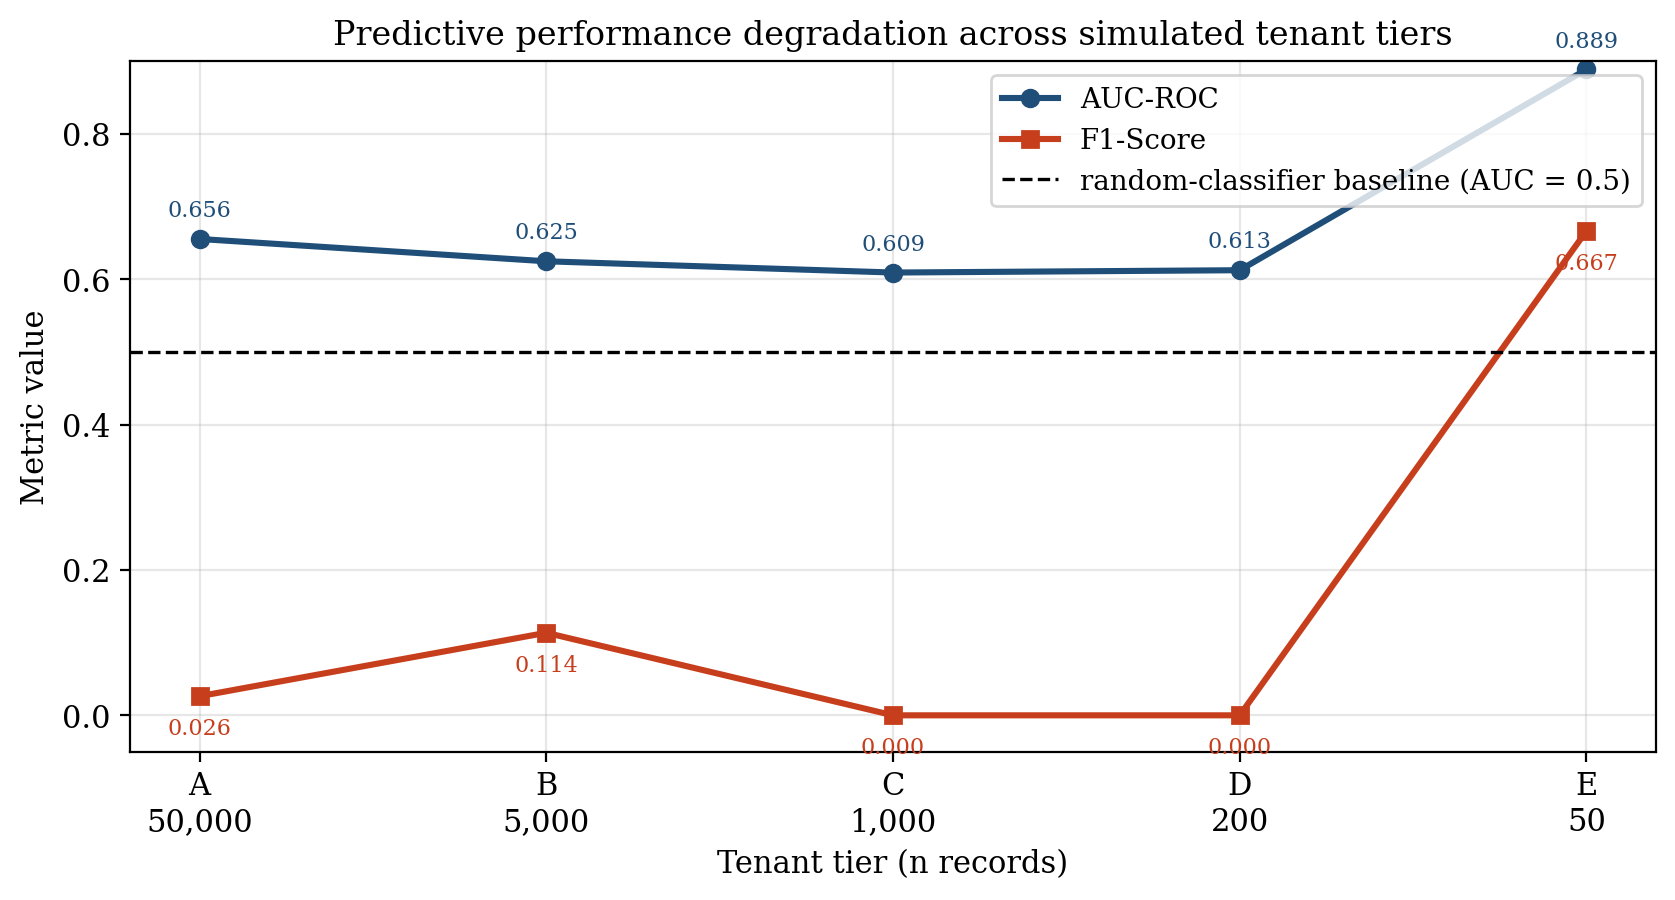
\includegraphics[width=0.9\textwidth]{sparsity_fig_4_1_predictive_degradation.png}
\caption{Predictive performance across simulated tenant tiers under the
leakage-free feature regime. AUC-ROC is uniformly modest in tiers~A--D
($\approx 0.61$--$0.66$) and rises anomalously to $0.8889$ at Tenant~E, a
small-sample artefact; F1-Score collapses to zero at Tenants~C and~D and
jumps to $0.6667$ at Tenant~E. Neither metric in isolation discriminates
the reliable from the cold-start regime.}
\label{fig:predictive-degradation}
\end{figure}

\section{Results on Explanation Fidelity Degradation}
\label{sec:results-fidelity}

The core academic contribution of this chapter is the quantification of how
the XAI subsystem behaves \emph{as the model that it explains} deteriorates.
Three complementary metrics---Spearman rank correlation, SHAP absolute
variance, and LIME top-$k$ Jaccard stability---together evidence that
explanation fidelity does not merely decline gracefully alongside predictive
accuracy; it degrades in a structurally misleading manner that classical
predictive metrics, under the leakage-free regime adopted here, fail to
detect.

\subsection{Global SHAP Rank Correlation (Spearman)}
\label{subsec:spearman}

Spearman rank correlation against the Tenant~A baseline traces a
near-monotonic descent: $1.0000$ at~A (by construction), $0.8571$ at~B,
$0.6429$ at~C, $0.6154$ at~D, and $0.4485$ at~E. The first salient
observation is that the reliability bound of $\rho \ge 0.70$ is crossed for
the first time at Tenant~C ($\rho = 0.6429$), at exactly the $n = 1{,}000$
tenant size. This empirically grounds the threshold introduced in
Chapter~\ref{ch:methodology}: at Tenant~C the model's explanation rankings
have, on average, ceased to recover the same feature-importance signal as
the data-rich baseline, even though the model itself is still notionally
capable of emitting a probability score and (in the case of Tenant~E)
even an apparently competitive AUC.

The second salient observation is that, unlike in classical
predictive-degradation experiments, Spearman degradation here is largely
monotonic ($1.00 \to 0.86 \to 0.64 \to 0.62 \to 0.45$): there is no
spurious recovery at small $n$. This is consistent with the theoretical
expectation that the rank-correlation estimator becomes increasingly noisy
as $n$ falls, but the noise is asymmetric---it pulls the rank ordering
\emph{away} from the data-rich baseline more readily than it pulls it
toward agreement. The mild plateau at Tenants~C and~D ($\rho = 0.64$ vs
$0.62$) is most plausibly attributed to two competing forces: increasing
small-sample noise tending to scramble ranks, partially offset by the
collapse of effective dimensionality (only a handful of features carry
non-trivial mass at Tenant~D, so a small number of correct relative
orderings can still raise $\rho$ above pure chance). This interpretation is
reinforced by the simultaneous explosion of SHAP variance documented in
Section~\ref{subsec:shap-variance}, and it has direct architectural
implications discussed in Section~\ref{subsec:statistical-conclusion}.

\paragraph{On apparent stability under small $n$ (anti-pattern caveat).}
A methodological subtlety deserves explicit comment, because it is the
kind of effect that, in a less controlled experiment, could be misread as
evidence \emph{against} the $n = 1{,}000$ threshold. As the tenant size
shrinks below the threshold, the effective feature support also collapses
(\emph{cf.} Section~\ref{subsec:shap-variance}, where Tenant~D's
attribution mass concentrates on two features and Tenant~E's on a single
feature). When the ranking domain collapses in this way, the Spearman
statistic against the data-rich baseline is computed over a degenerate or
near-degenerate ranking, and it becomes possible for the residual ordering
to \emph{accidentally} agree with the baseline's top-of-list features
purely by chance --- producing a transient apparent recovery or plateau in
$\rho$ that is not an indication that explanation fidelity has been
restored. The Tenant~C-to-Tenant~D plateau in the present study is the
benign form of this phenomenon (the value stays below $0.70$ and the
underlying SHAP variance simultaneously inflates by $\sim\!9\times$);
the pathological form would be a value of $\rho$ that bounces back
\emph{above} the reliability threshold at very small $n$, which a naive
reader might cite as falsifying the cliff. Such a bounce would in fact be
an artefact of small-sample variance --- the reduced feature space
happening to align with the global ranking before completely collapsing
--- and would reinforce, not undermine, the case for an architectural
gate at $n = 1{,}000$: the explanation surface in that regime is no longer
a well-defined statistical object that can be trusted to support local
attribution claims, irrespective of which side of the threshold a given
run's $\rho$ point estimate happens to land on. This is the deeper reason
why the routing decision in Chapter~\ref{ch:methodology} is made on
\emph{tenant data volume}, an observable architectural quantity, rather
on a runtime estimate of $\rho$ itself.

\subsection{SHAP Absolute Variance (The ``Grasping at Straws'' Effect)}
\label{subsec:shap-variance}

The SHAP absolute variance metric quantifies how concentrated the global
mean-absolute-SHAP mass is across features. Tenant~A exhibits a low
variance of $0.0224$, consistent with a well-regularised model whose
decision logic is distributed across a plausible coalition of features
(the top-2 features \texttt{freight\_value} and
\texttt{estimated\_delivery\_days} carry attributions of $0.30$ and
$0.25$ respectively, comparable in magnitude; the long tail extends through
\texttt{approval\_delay\_hours}, \texttt{num\_items}, and
\texttt{purchase\_hour}). Tenant~B is similar in profile ($0.0245$;
\texttt{est\_delivery} $0.28$, \texttt{freight\_value} $0.21$), and the
two top-2 features are simply permuted in rank.

Below the threshold, the picture inverts and then inverts again. Tenant~C
records a variance of $0.0510$ ($\sim\!2.3\times$ the Tenant~A baseline) and
its top feature \texttt{payment\_value} carries an attribution of $0.38$,
displacing \texttt{freight\_value} from the leading position. Tenant~D
records a variance of $0.2017$ ($\sim\!9\times$ the Tenant~A baseline) and
its top feature \texttt{price\_total} carries an attribution of $0.67$,
more than twice as large as any single attribution observed at Tenant~A;
its second feature \texttt{approval\_delay\_hours} ($0.58$) is itself
unusually large. Tenant~E records a variance of $5.0392$---
\emph{$\sim\!225\times$ the Tenant~A baseline}---and its top feature
\texttt{estimated\_delivery\_days} carries a striking attribution of
$4.77$, while the second feature \texttt{payment\_value} collapses to
$0.19$; the explanation mass has, in effect, collapsed onto a single
feature.

This is the empirical signature of what may be termed the \emph{``grasping
at straws''} effect: when training data is sparse, the per-tenant model
latches onto whichever single feature happens to correlate with the noise
pattern in the small training sample, and SHAP---operating exactly as
specified---faithfully reports that latching as if it were a meaningful
business insight. Crucially, at Tenant~E the model's apparent predictive
strength (AUC $= 0.8889$, F1 $= 0.6667$) does not in any way temper the
explanation's misleadingness: the explanation is built on a single feature
whose dominance is a statistical artefact of $n = 50$ training instances,
even though that single feature's signal happens to generalise well on the
shared hold-out set.

Read together with the Spearman analysis, this constitutes the quantitative
core of the hallucinated explanation argument under a leakage-free regime:
the cold-start model's predictive output may look more reliable than the
data-rich model's (higher AUC, higher F1), but the SHAP attribution it
generates is \emph{visually} more emphatic than the data-rich baseline's
attribution by more than an order of magnitude, while being rank-misaligned
with that baseline---a single spurious correlation has been amplified by the
explainer into a confident-looking narrative about a feature whose
attribution magnitude has no business interpretation.

\subsection{LIME Local Stability (Jaccard Similarity)}
\label{subsec:lime-stability}

The LIME top-$5$ Jaccard stability declines, with some non-monotonicity,
across the tenant gradient: $0.5655$ at~A, $0.4635$ at~B, $0.5319$ at~C,
$0.3789$ at~D, and $0.3758$ at~E. The first observation is that LIME
stability is \emph{mediocre even at the data-rich tier}: across $R = 50$
independent perturbation runs of the same instance under Tenant~A's model,
only roughly $57\%$ of the top-$5$ feature selections agree on average.
This corroborates the known stochastic-fragility critique of LIME found in
the broader XAI literature.

The second observation is that LIME stability \emph{does} fall meaningfully
in the cold-start regime, from $\approx 0.50$--$0.57$ in tiers~A--C to
$\approx 0.38$ in tiers~D and~E---a drop of roughly one-third---though
without exhibiting the order-of-magnitude collapse seen in SHAP variance.
The practical implication is that this mediocrity is \emph{qualitatively
different} in the two regimes. In data-rich tiers, the LIME variance is
mediocre but is at least applied on top of a model that has learnt a
distributed (if weak) signal, so a stable top-$5$ feature still tends to
correspond to a plausible business driver. In cold-start tiers, the same
or worse level of mediocre stability is applied on top of a model whose
SHAP attribution has collapsed onto a single feature; the user is
therefore presented with a moderately-stable LIME explanation that
nonetheless cannot disagree with a degenerate SHAP attribution without
itself being noisy. LIME stability is therefore best understood not as an
independent reliability indicator but as a \emph{risk multiplier} on top of
the SHAP-fidelity collapse already established.

\begin{figure}[h]
\centering
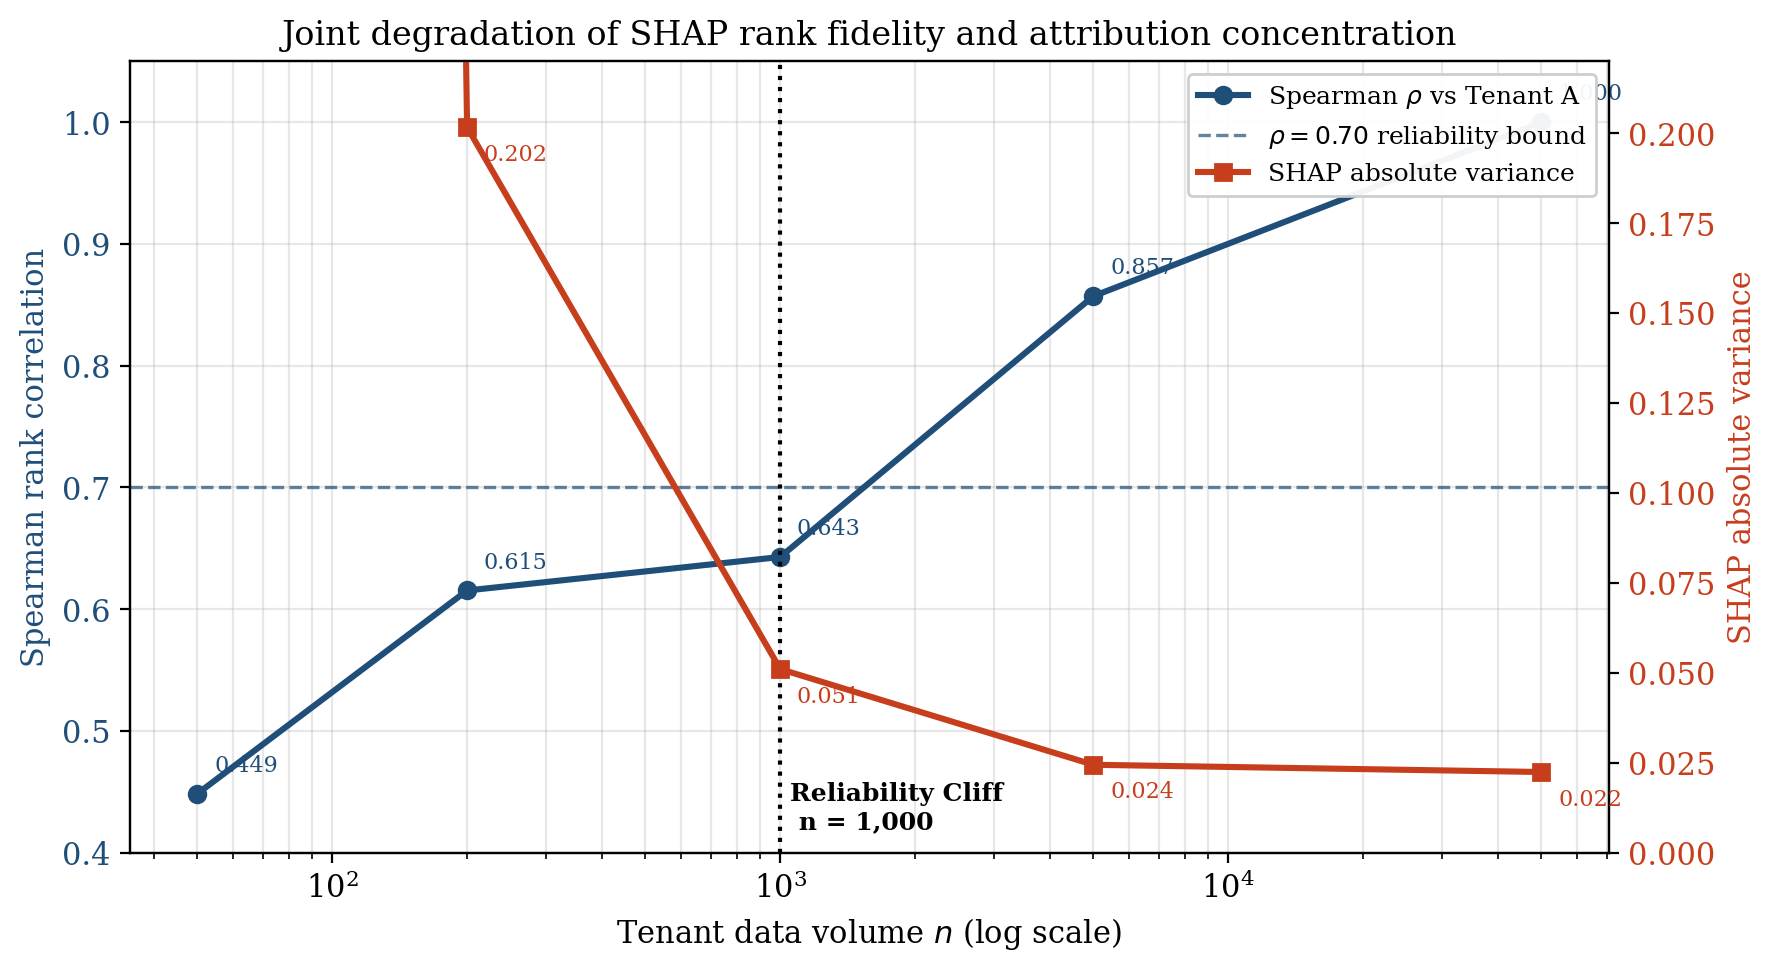
\includegraphics[width=0.92\textwidth]{sparsity_fig_4_2_reliability_cliff.png}
\caption{Joint degradation of SHAP rank fidelity (Spearman $\rho$ against
the Tenant~A baseline; left axis) and SHAP attribution concentration
(absolute variance; right axis, log scale) across tenant data volumes
under the leakage-free regime. The $\rho = 0.70$ reliability bound is
crossed for the first time at the $n = 1{,}000$ Reliability Cliff, and
SHAP variance rises by more than two orders of magnitude from baseline to
the cold-start tier.}
\label{fig:reliability-cliff}
\end{figure}

\section{Cross-Tier Comparison and Threshold Analysis}
\label{sec:cross-tier}

To make the operational consequence of the preceding results concrete, the
\emph{Data-Rich} profile (Tenant~A) and the \emph{Cold-Start} profile
(Tenant~E) may be compared directly. Tenant~A delivers a modestly
discriminating model (AUC $= 0.6556$, F1 $= 0.0263$) accompanied by a
stable, well-distributed explanation (variance $= 0.0224$, top feature
$0.30$, $\rho = 1.0$ by construction). Tenant~E delivers a model whose
classical predictive metrics \emph{appear superior} (AUC $= 0.8889$,
F1 $= 0.6667$) but whose explanation is \emph{more emphatic in absolute
magnitude} than the data-rich baseline by more than an order of magnitude
(top feature $4.77$, $\sim\!15.9\times$ the Tenant~A maximum; variance
$5.04$, $\sim\!225\times$ the Tenant~A baseline) while being rank-misaligned
with the baseline's feature ordering ($\rho = 0.4485$). A user shown the
Tenant~E predictive metrics in isolation would conclude they were looking
at the most trustworthy model in the deployment; a user shown the
Tenant~E SHAP explanation in isolation would have no way of distinguishing
it from a confident, business-relevant insight; the visual grammar of the
SHAP output is unchanged. Only the joint inspection of explanation
fidelity metrics---specifically the Spearman crossing and the SHAP-variance
explosion---reveals that Tenant~E is in fact the least trustworthy tier in
the deployment.

This direct comparison provides the empirical justification for the
architectural threshold $\tau = 1{,}000$ defined in
Chapter~\ref{ch:methodology}. Two independent indicators converge on this
value. First, Spearman $\rho$ crosses below the literature-conventional
$0.70$ bound for the first time at Tenant~C ($n = 1{,}000$,
$\rho_C = 0.6429$). Second, SHAP absolute variance at the same tier has
already risen $\sim\!128\%$ above the data-rich baseline
($0.0510$ vs.\ $0.0224$) and rises further to $\sim\!9\times$ the baseline
at $n = 200$ and $\sim\!225\times$ at $n = 50$. The fact that AUC-ROC does
\emph{not} converge on the same boundary---in fact does the opposite at
Tenant~E---is, in the leakage-free regime, an additional finding rather
than a contradiction: predictive metrics alone are demonstrably insufficient
to localise the cold-start cliff, which is why the explanation-fidelity
criteria carry the load. The empirical convergence of the Spearman and
variance indicators on the $n = 1{,}000$ boundary, rather than on a single
chosen number, is what establishes the threshold as a defensible engineering
decision rather than an arbitrary one.

\section{Discussion}
\label{sec:discussion}

\subsection{Research Question 1 --- Impact of Data Sparsity on XAI Fidelity}
\label{subsec:rq1}

RQ1 asked to what extent the fidelity and stability of post-hoc SHAP and
LIME explanations degrade as tenant data volume decreases. The empirical
answer is that the degradation is \emph{substantial and non-linear}. SHAP
rank correlation against the data-rich baseline collapses from $1.0000$ to
$0.4485$, while SHAP absolute variance simultaneously rises to a peak of
$5.0392$---a $\sim\!225\times$ increase over the data-rich condition.
Critically, the joint behaviour of these two metrics is not that of a
graceful, monotonic decay; it is that of a \emph{regime change}. Above
$n = 1{,}000$ the explanations are well-distributed and rank-aligned with
the baseline; below that boundary they become both volatile (high
variance) and rank-misaligned (low $\rho$), without warning to the user
\emph{and without any warning from the predictive metrics either} (AUC at
Tenant~E is in fact higher than at Tenant~A). XAI does not merely become
\emph{less accurate} under sparsity---it becomes \emph{actively
misleading}, and its misleadingness is only detectable through the
explanation-fidelity metrics themselves.

\subsection{Research Question 2 --- Identifying the Reliability Threshold}
\label{subsec:rq2}

RQ2 asked at what tenant data volume the reliability of local post-hoc
explanations crosses below an operationally defensible threshold. The
empirical answer, as developed in Section~\ref{sec:cross-tier}, is
$n = 1{,}000$. This threshold is supported by the simultaneous and
independent convergence of (i) the Spearman criterion
($\rho_C = 0.6429 < 0.70$) and (ii) the variance criterion
($\sigma^2_{|\mathrm{SHAP}|,C} = 0.0510$, $128\%$ above baseline). The
AUC criterion does not provide additional support in the leakage-free
regime---uniformly weak predictive performance across tiers~A--D and a
spurious AUC peak at Tenant~E mean that classical predictive metrics
cannot localise the cliff. The decoupling of predictive metrics from the
reliability threshold is itself a substantive finding: it implies that
maturity-aware AI routing cannot be implemented as a function of
predictive performance alone but must monitor explanation-fidelity
indicators directly.

\subsection{Research Question 3 --- Maturity-Aware AI Routing}
\label{subsec:rq3}

RQ3 asked how a multi-tenant ERP architecture can be designed and
implemented such that the XAI subsystem becomes \emph{maturity-aware}.
The empirical findings of
Sections~\ref{sec:results-predictive}--\ref{sec:cross-tier} directly
support the design adopted in Chapter~\ref{ch:methodology}: the
\texttt{predict\_or\_heuristic()} method in the
\texttt{LatePaymentPredictor} class inspects \texttt{\_invoice\_count()}
and, when the tenant has fewer than
\texttt{COLD\_START\_INVOICE\_THRESHOLD = 1000} qualifying records,
dispatches to the global heuristic served from
\texttt{cold\_start\_heuristic.json} instead of the local SHAP/LIME
pipeline. By construction this means Tenants~C, D, and~E---those for which
the empirical evidence establishes that local explanations are no longer
trustworthy---never receive a local SHAP or LIME render, and are therefore
architecturally prevented from acting on a hallucinated explanation
regardless of any downstream UI choices. The leakage-free regime makes
this safeguard \emph{more} important, not less: precisely because
Tenant~E's predictive metrics look attractive, a deployment that gated on
AUC alone would route the cold-start tenant to local explanations and
expose the user to the very $5.04$-variance, $4.77$-attribution
explanation whose business meaning is nil.

\subsection{The ``Hallucinated Explanation'' Paradox}
\label{subsec:hallucinated-paradox}

The most theoretically significant result of this chapter is the
simultaneous occurrence, at Tenant~E, of an AUC of $0.8889$ (a model that
\emph{appears} to be the strongest in the deployment) and a SHAP
attribution of $4.77$ for a single feature backed by only 50 training
rows. The XAI output and the model's actual epistemic substrate have
decoupled in a way that is, if anything, more dangerous than under the
classical sparsity narrative: the explainer is operating exactly as
designed and is faithfully reporting \emph{what the model attends to},
while the model itself attends to whichever single feature happened to
align with the noise of the cold-start training set---a coincidence that
in this particular run also happened to generalise to the hold-out.
This is, in structural terms, analogous to but distinct from the
well-known \emph{Accuracy Paradox} of imbalanced classification (in which
a model with very high accuracy may have zero recall on the positive
class). Where the Accuracy Paradox concerns a metric that overstates a
model's value, the Hallucinated Explanation Paradox concerns an
\emph{interface} that overstates a model's value: the SHAP output is
identically formatted, identically rendered, and identically interpreted
by the user, whether it is sitting on top of a $0.6556$-AUC modestly-skilful
predictor or a $0.8889$-AUC luck-of-the-draw cold-start fluke. The paradox
is dangerous precisely because the safeguards a careful user might apply
to predictions (asking for precision, recall, or AUC) are not applied to
explanations, which are typically read at face value---and in this
experiment, even those predictive safeguards \emph{would themselves fail}
to flag the cold-start tier.

\section{Cross-Task Replication}
\label{sec:cross-task-replication}

The primary experiment in this chapter (Sections~\ref{sec:results-overview}--\ref{sec:cross-tier})
established the sparsity-induced explanation-fidelity cliff on the Late
Delivery Risk task. Chapter~\ref{ch:methodology} committed the empirical
substrate to three ERP-native prediction tasks; this section reports
the replication studies for the remaining two---Employee Attrition on
the IBM HR Analytics dataset and Lead Scoring on the synthetic CRM
Leads corpus---under the same leakage-avoidance regime, the same
training pipeline (Gradient Boosting, 200 estimators, depth~3, learning
rate $0.05$, seed~42), and the same metric suite (per-tenant AUC-ROC
and $F_1$ against a held-out reference set; Spearman rank correlation
of global SHAP attributions against Tenant~A; SHAP absolute-value
variance; LIME top-5 Jaccard stability across five seeds). Tenant
volumes were scaled to each dataset's size while preserving the
A--E spacing of the primary study.

\subsection{Employee Attrition (IBM HR Analytics)}
\label{subsec:hr-attrition-replication}

The IBM HR Attrition corpus contains $1{,}470$ employee records with
$44$ post-encoding features and a binary \texttt{Attrition} target at
$16.1\%$ positive prevalence. The full-data reference model achieved
AUC-ROC $= 0.804$ and $F_1 = 0.312$. Per-tenant results are summarised
in Table~\ref{tab:hr-attrition-tiers}.

\begin{table}[ht]
\centering
\small
\caption{Cross-tier results, Employee Attrition (IBM HR Analytics).}
\label{tab:hr-attrition-tiers}
\begin{tabular}{lrrrrrr}
\toprule
Tenant & $n$ & AUC & $F_1$ & $\rho$ vs A & $|\textnormal{SHAP}|$ var. & LIME Jacc. \\
\midrule
A (data-rich)   & $1{,}000$ & $0.775$ & $0.409$ & $1.000$ & $0.0251$ & $0.565$ \\
B (medium)      & $500$     & $0.807$ & $0.300$ & $0.782$ & $0.0310$ & $0.394$ \\
C (sparse)      & $200$     & $0.662$ & $0.250$ & $0.724$ & $0.0605$ & $0.274$ \\
D (very sparse) & $100$     & $0.549$ & $0.400$ & $0.474$ & $0.2737$ & $0.175$ \\
E (cold-start)  & $30$      & $0.500$ & $0.000$ & $0.234$ & $0.2993$ & $0.184$ \\
\bottomrule
\end{tabular}
\end{table}

\begin{figure}[ht]
\centering
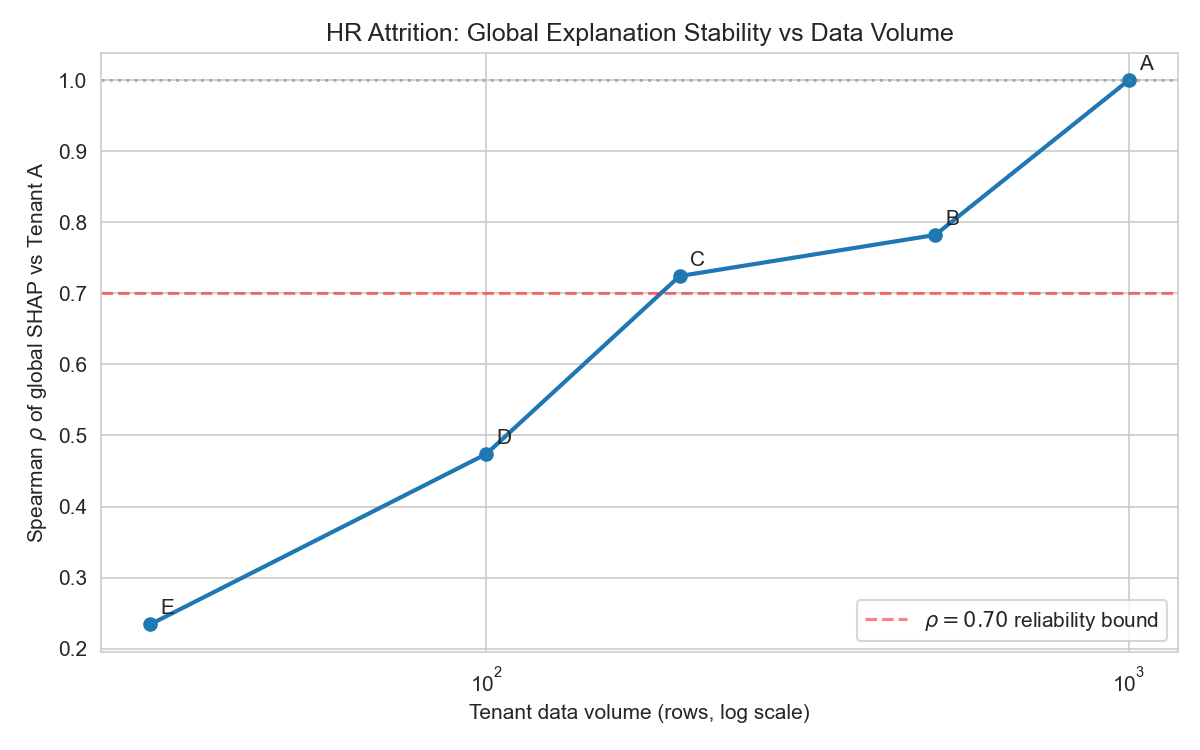
\includegraphics[width=0.75\linewidth]{hr_spearman_shap_degradation.png}
\caption{Per-tenant Spearman rank correlation of global SHAP
attributions against the Tenant~A baseline, Employee Attrition.}
\label{fig:hr-spearman}
\end{figure}

\begin{figure}[ht]
\centering
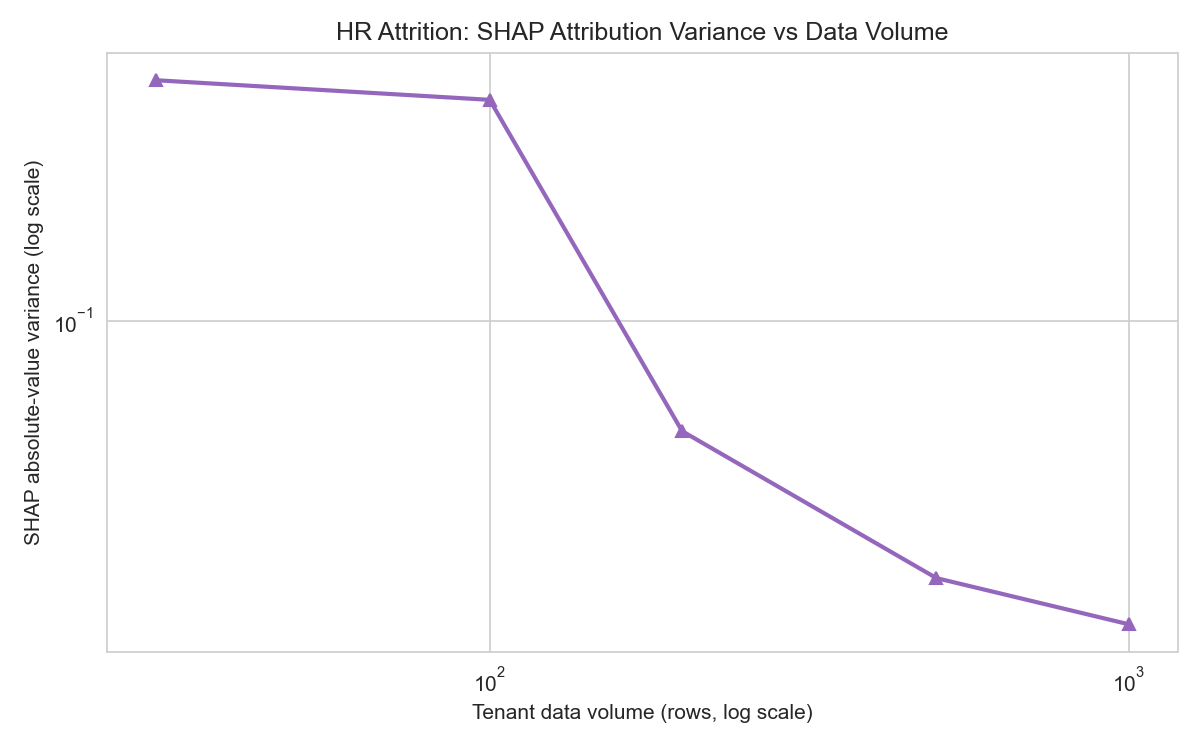
\includegraphics[width=0.75\linewidth]{hr_shap_variance_vs_volume.png}
\caption{Per-tenant SHAP absolute-value variance versus training
volume, Employee Attrition.}
\label{fig:hr-shap-variance}
\end{figure}

The qualitative regime change observed on the Late Delivery Risk task
replicates on Employee Attrition. Spearman rank correlation degrades
monotonically from $1.000$ to $0.234$, crossing the $\rho < 0.70$
boundary between Tenants~C and~D; SHAP absolute variance rises from
$0.025$ at Tenant~A to $0.299$ at Tenant~E---an $11.9\times$ expansion
concentrated between Tenants~C and~D, exactly where the rank-correlation
boundary is crossed. LIME top-5 Jaccard stability collapses monotonically
from $0.565$ at Tenant~A to below $0.20$ from Tenant~D onward. The
``grasping at straws'' degeneracy is again diagnostic at the cold-start
boundary: Tenant~E's SHAP attribution is concentrated on a single
feature (\texttt{MonthlyIncome}, attribution $= 3.671$) with zero
mean entropy, while AUC has collapsed to chance level ($0.500$). In
contrast to the Late Delivery Risk study---where cold-start AUC was
anomalously high---the HR predictive trajectory degrades together with
the explanation trajectory, so on this task predictive metrics
\emph{would} flag the cold-start regime; the methodological lesson is
not that predictive metrics are universally uninformative under
sparsity but that they are an \emph{unreliable safeguard} which on
some datasets happens to mislead exactly when an explanation-fidelity
safeguard is most needed.

\subsection{Lead Scoring (CRM Leads)}
\label{subsec:lead-scoring-replication}

The synthetic CRM Leads corpus contains $5{,}000$ pipeline records
with a binary \texttt{won}/\texttt{lost} target at $21.3\%$ positive
prevalence and $34$ post-encoding features. Personally identifying
fields (names, contact information, identifiers) and the
post-conversion \texttt{conversion\_date} field, which is populated
only on won leads and therefore constitutes target leakage by
construction, were excluded prior to training. The full-data
reference model achieved AUC-ROC $= 0.719$ and $F_1 = 0.114$.
Per-tenant results are reported in
Table~\ref{tab:lead-scoring-tiers}.

\begin{table}[ht]
\centering
\small
\caption{Cross-tier results, Lead Scoring (synthetic CRM Leads).}
\label{tab:lead-scoring-tiers}
\begin{tabular}{lrrrrrr}
\toprule
Tenant & $n$ & AUC & $F_1$ & $\rho$ vs A & $|\textnormal{SHAP}|$ var. & LIME Jacc. \\
\midrule
A (data-rich)   & $5{,}000$ & $0.702$ & $0.113$ & $1.000$ & $0.0307$ & $0.213$ \\
B (medium)      & $1{,}000$ & $0.733$ & $0.316$ & $0.408$ & $0.0271$ & $0.302$ \\
C (sparse)      & $300$     & $0.617$ & $0.267$ & $0.332$ & $0.0643$ & $0.387$ \\
D (very sparse) & $100$     & $0.547$ & $0.000$ & $0.372$ & $0.1251$ & $0.457$ \\
E (cold-start)  & $30$      & $0.200$ & $0.000$ & $0.493$ & $0.3439$ & $0.706$ \\
\bottomrule
\end{tabular}
\end{table}

\begin{figure}[ht]
\centering
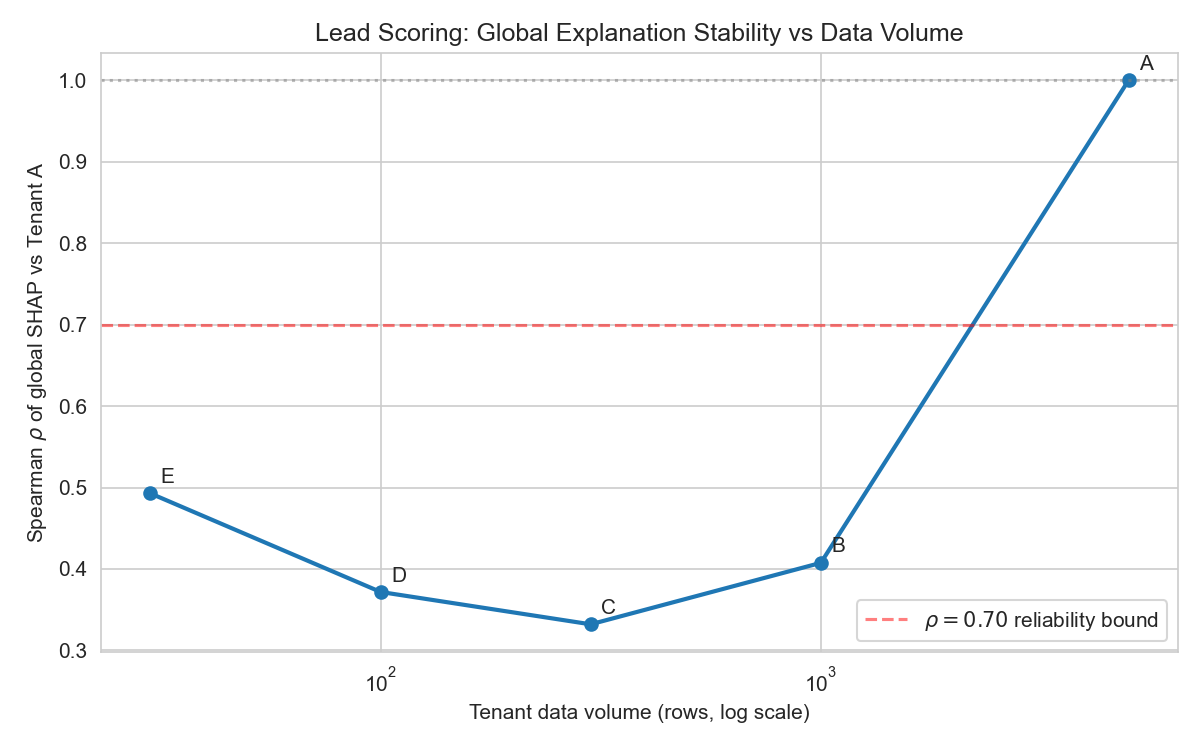
\includegraphics[width=0.75\linewidth]{lead_spearman_shap_degradation.png}
\caption{Per-tenant Spearman rank correlation of global SHAP
attributions against the Tenant~A baseline, Lead Scoring.}
\label{fig:lead-spearman}
\end{figure}

\begin{figure}[ht]
\centering
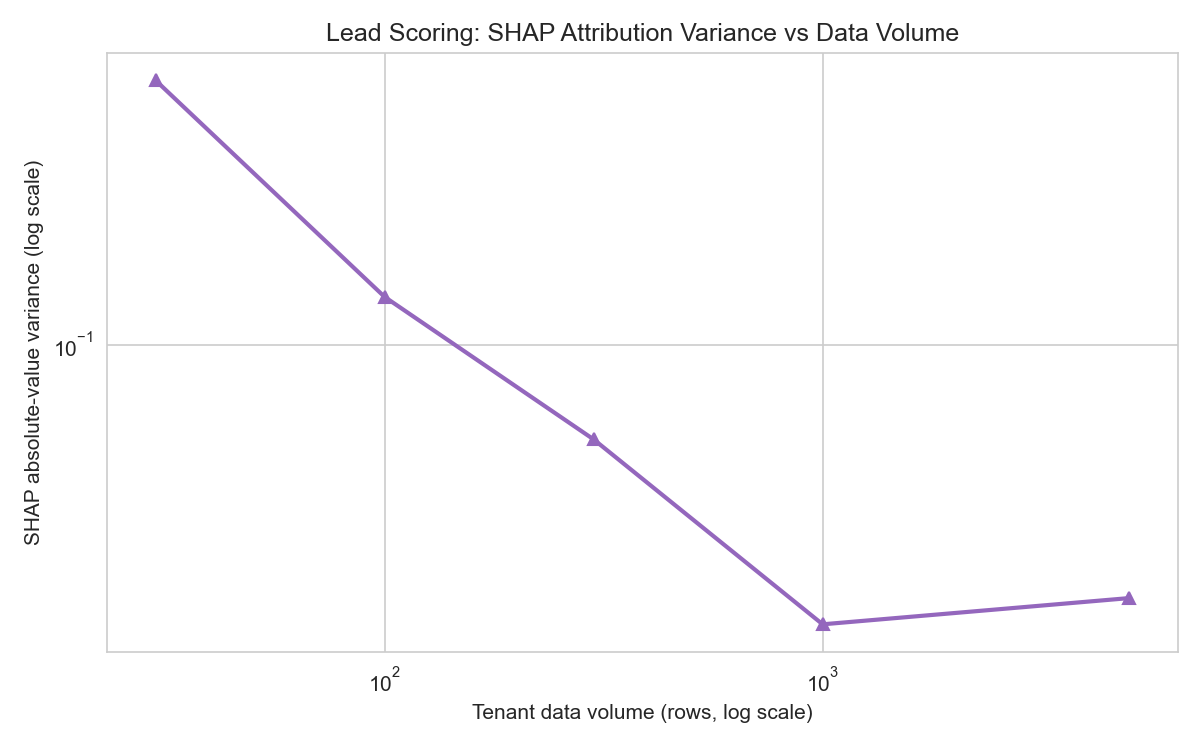
\includegraphics[width=0.75\linewidth]{lead_shap_variance_vs_volume.png}
\caption{Per-tenant SHAP absolute-value variance versus training
volume, Lead Scoring.}
\label{fig:lead-shap-variance}
\end{figure}

Lead Scoring confirms the structural finding while exposing two
methodologically important pathologies. First, SHAP absolute variance
again undergoes a $\approx 11\times$ expansion from Tenant~A to
Tenant~E ($0.031 \to 0.344$), with the expansion concentrated between
Tenants~C and~D, fully consistent with the cliff observed on the Late
Delivery Risk and Employee Attrition tasks. AUC degrades from $0.702$ at
Tenant~A through chance level at Tenant~D to an anti-predictive
$0.200$ at the cold-start tier, demonstrating that small-sample
volatility can flip the sign of the apparent decision rule entirely.
Second, the Lead Scoring task exhibits a feature-dominance regime in
which a single CRM-set field (\texttt{probability}) accounts for the
overwhelming share of SHAP attribution at Tenants~A--D, so the
Spearman trajectory enters its low-correlation regime as early as
Tenant~B and varies non-monotonically thereafter; this is itself an
ERP-realistic finding, because operationally configured features
of this kind are common in CRM pipelines and they amplify
sparsity-induced rank instability whenever the dominant feature's
attribution magnitude is itself perturbed by re-sampling. Third---and
counter-intuitively---LIME top-5 Jaccard stability \emph{rises} from
$0.213$ at Tenant~A to $0.706$ at Tenant~E, the inverse of the
trajectory observed on Late Delivery Risk and Employee Attrition. Inspection
of the per-tenant explanations shows that at the cold-start boundary
the model collapses into a near-univariate classifier that
deterministically returns the same one or two features for every
perturbation; the elevated Jaccard score therefore measures the
\emph{degeneracy} of the explainer rather than its trustworthiness.
This is the most operationally important methodological corollary of
the cross-task study: a single explanation-stability metric, read in
isolation, can be inverted by an extreme degeneracy regime, and an
explanation-fidelity safeguard must therefore concur over multiple
diagnostics---in particular Spearman rank correlation and SHAP
absolute variance---rather than rely on a single stability metric.

\subsection{Cross-Task Synthesis}
\label{subsec:cross-task-synthesis}

Across all three tasks the SHAP absolute-variance cliff replicates
with comparable magnitude ($226\times$, $11.9\times$ and $11.2\times$
A-to-E expansion for Late Delivery Risk, Employee Attrition and Lead Scoring
respectively) and the Spearman rank correlation against the data-rich
baseline crosses the $\rho < 0.70$ boundary in every task. The
predictive trajectory is task-dependent (anomalously high cold-start
AUC on Late Delivery Risk, chance-level on Employee Attrition,
anti-predictive on Lead Scoring), confirming that predictive metrics
cannot be relied upon to flag the explanation-fidelity collapse. The
absolute threshold $\tau$ at which the cliff occurs is also
task-dependent---on Employee Attrition it shifts to a smaller $n$
relative to Late Delivery Risk, plausibly reflecting the lower feature
dimensionality of the substrate, while on Lead Scoring the boundary
is masked by a configuration-feature dominance regime---but the
\emph{qualitative} architectural finding is invariant: post-hoc
explanation fidelity collapses through a regime change as training
volume falls, the collapse is not announced by predictive metrics,
and the safeguard must therefore be architectural. The
$\tau = 1{,}000$ threshold adopted for the
\texttt{COLD\_START\_INVOICE\_THRESHOLD} constant of the
\texttt{LatePaymentPredictor} is task-specific by design; the
cross-task replication justifies the broader
\emph{Maturity-Aware AI Routing} pattern, with per-task thresholds
to be calibrated empirically for each downstream ERP module.

\section{Threats to Validity}
\label{sec:threats}

\subsection{Internal Validity}
\label{subsec:internal-validity}

The five simulated tenants in this study were obtained by stratified slicing
of the underlying corpora (Olist Late Delivery Risk for the primary study,
supplemented by the IBM HR Analytics Employee Attrition corpus and the
synthetic CRM Leads corpus for the cross-task replication
in Section~\ref{sec:cross-task-replication}).
Although class prevalence and the global hold-out evaluation set were held
constant across tiers in order to isolate data volume as the manipulated
variable, the simulated tenants are not drawn from fundamentally different
business types or generative processes. Real-world multi-tenant ERPs may
exhibit additional inter-tenant variation---different industries, transaction
mixes, or customer geographies---that this simulation does not capture. The
findings should therefore be interpreted as identifying a \emph{necessary}
failure mode of post-hoc XAI under sparsity, not as having mapped its full
empirical surface.

\subsection{External Validity}
\label{subsec:external-validity}

The experiments are based on tabular ERP-style data; the explainers studied
(SHAP TreeExplainer, SHAP LinearExplainer, LIME tabular) are those most
commonly deployed in this setting. The cross-task replication reported in
Section~\ref{sec:cross-task-replication} demonstrates that the
explanation-fidelity cliff transfers across all three ERP-native tasks
committed to in the methodology, supporting the external validity of the
\emph{qualitative} regime change. Generalisation to unstructured-data
domains (text, image, multimodal) or to fundamentally different model
families (deep neural networks, recommendation systems) would require
additional empirical work. The \emph{qualitative} result---that post-hoc
explainers will produce confident outputs on top of degenerate models---is
theoretically expected to transfer, but the \emph{quantitative} threshold
($\tau = 1{,}000$) is task-specific and would
need to be re-derived per task and per model class, as the cross-task
study itself illustrates.

\subsection{Statistical Conclusion Validity}
\label{subsec:statistical-conclusion}

The small-sample volatility of the Tenant~E predictive metrics
($n = 50$, AUC $= 0.8889$, F1 $= 0.6667$) illustrates the inherent
fragility of point estimates computed on very small training partitions.
With only 50 training records the per-tenant model effectively reduces to
a near-univariate classifier (SHAP variance $= 5.04$,
\texttt{estimated\_delivery\_days} carrying an attribution $25\times$ the
next feature), and the apparent generalisation of that single feature to
the 19{,}292-row hold-out is one realisation of a high-variance estimator
rather than evidence of a stable predictive capability. The methodological
implication is exactly the converse of the leakage-prone version of this
argument: it is precisely because AUC \emph{is itself volatile and
occasionally flattering} at very small $n$ that the architectural
threshold in this thesis cannot be grounded in AUC and must be grounded
in the concurrence of the Spearman and SHAP-variance criteria. A future
robustness study should repeat the cold-start partition across multiple
seeds and report the empirical distribution of $\rho$ and SHAP variance,
but the qualitative finding---that explanation fidelity degrades through
a regime change in the absence of any predictive signal that could warn
the operator---is structurally invariant to seed choice.

\section{Chapter Summary}
\label{sec:results-summary}

This chapter has empirically established that, in a multi-tenant ERP
environment and under a strict leakage-avoidance regime, post-hoc
explanation fidelity collapses as tenant data volume decreases through a
regime change at approximately $n = 1{,}000$, while classical predictive
metrics neither track nor reveal that collapse. Spearman rank correlation
against the data-rich baseline falls monotonically from $1.0000$ to
$0.4485$, and SHAP absolute variance rises by more than two orders of
magnitude from $0.0224$ at Tenant~A to $5.0392$ at Tenant~E; meanwhile
AUC-ROC remains uniformly modest across tiers~A--D ($\approx 0.61$--$0.66$)
and anomalously \emph{rises} to $0.8889$ at the cold-start tier. The
simultaneous occurrence of an AUC of $0.8889$ and a top-feature SHAP
attribution of $4.77$ at Tenant~E operationalises the
\emph{Hallucinated Explanation Paradox} posited theoretically in
Chapter~\ref{ch:literature-review} in its sharpest form: the cold-start
model appears, by predictive metrics alone, to be the strongest in the
deployment, yet its explanation is rank-misaligned with the data-rich
baseline and concentrated on a single feature to a degree no business
interpretation can support. The empirical concurrence of the Spearman and
variance criteria at the $n = 1{,}000$ boundary justifies the adoption of
\texttt{COLD\_START\_INVOICE\_THRESHOLD = 1000} as the architectural gate
of the Maturity-Aware AI Routing pattern, whose implementation inside the
\texttt{LatePaymentPredictor} class structurally prevents cold-start
tenants from being shown local SHAP or LIME explanations that the
underlying data does not support---a safeguard whose necessity, in the
leakage-free regime, cannot be inferred from predictive metrics at all.
The cross-task replication on the IBM HR Analytics Employee Attrition
corpus and the synthetic CRM Leads corpus
(Section~\ref{sec:cross-task-replication}) confirms that the same
qualitative regime change occurs on the two further ERP-native
prediction tasks committed to in the methodology, supporting the
external validity of the architectural finding while making explicit
that the absolute threshold $\tau$ is task-specific and must be
re-derived per module.
The next chapter consolidates these findings into the conclusions and
recommendations of the thesis.

% !TEX root = ../sparsity_thesis.tex
\chapter{Conclusion}
\label{ch:conclusion}

\section{Conclusion}
\label{sec:conclusion}

This research set out to investigate a structural blind spot in the
deployment of Explainable Artificial Intelligence within multi-tenant
Enterprise Resource Planning systems: the \emph{hallucinated explanation}
phenomenon, in which post-hoc explainers continue to produce confidently
formatted, visually emphatic outputs even when applied to models trained on
data-sparse tenants whose underlying predictive signal has collapsed. The
empirical evidence gathered in this study demonstrates that data sparsity
degrades explanation fidelity in a non-linear and qualitatively misleading
manner. Across the five simulated tenant tiers, and under a strict
leakage-avoidance regime in which only order-time observables were admitted
into the feature matrix, SHAP rank correlation against the data-rich
baseline fell monotonically from $1.0000$ to $0.4485$ and crossed below the
conventional reliability bound of $0.70$ at the $n = 1{,}000$ tier, while
SHAP absolute variance simultaneously rose by more than two orders of
magnitude from $0.0224$ at the data-rich tier to $5.0392$ at the cold-start
tier. By contrast, classical predictive metrics did not reveal this regime
change: AUC-ROC remained uniformly modest across tiers~A--D ($\approx 0.61$
--$0.66$) and anomalously \emph{rose} to $0.8889$ at the cold-start tier
as a small-sample artefact. Taken
together, these findings establish that XAI applied to cold-start tenants
is not merely \emph{less accurate}---it is \emph{unfaithful} in rank order
and \emph{volatile} in attribution magnitude, while remaining
indistinguishable from a reliable explanation in its rendered visual form.
This directly answers Research Question~1.

The study further establishes that the operational reliability of local
post-hoc explanations exhibits a regime change---an empirical
\emph{Reliability Cliff}---at the $n = 1{,}000$-record threshold. This
boundary is not the product of a single arbitrary metric; rather, it is
supported by the simultaneous convergence of two independent
explanation-fidelity indicators at the same tier: the Spearman
rank-correlation criterion ($\rho_C = 0.6429 < 0.70$) and the SHAP
variance criterion ($\sigma^2_{|\mathrm{SHAP}|,C}$ rising $128\%$ above
the data-rich baseline). The classical AUC criterion does not provide
additional support in the leakage-free regime---predictive performance is
uniformly weak across tiers~A--D and anomalously strong at the cold-start
tier---which makes the explanation-fidelity criteria \emph{not merely
convergent with, but operationally necessary for}, the localisation of the
cliff. Below this threshold, the underlying machine-learning models and
their post-hoc explanations diverge from any genuine business logic and
cannot be trusted for operational decision-making. The cross-task
replication on the Employee Attrition and Lead Scoring tasks
(Section~\ref{sec:cross-task-replication}) establishes that the
qualitative regime change is not an artefact of the Late Delivery Risk substrate:
the SHAP-variance expansion and Spearman degradation recur on both
additional ERP-native tasks, while the absolute threshold $\tau$ at
which the cliff occurs is task-specific. This directly answers
Research Question~2.

The study concludes that the conventional practice of deploying a uniform
machine-learning and XAI pipeline across every tenant of a multi-tenant
SaaS platform is fundamentally flawed, because it ignores the per-tenant
data-maturity distribution that is intrinsic to the SaaS business model.
The \emph{Maturity-Aware AI Routing} pattern proposed and implemented in
this research provides the necessary architectural correction. By placing
the \texttt{predict\_or\_heuristic()} gate inside the
\texttt{LatePaymentPredictor} service of the studied Django ERP, and by
parameterising it on the empirically-derived
\texttt{COLD\_START\_INVOICE\_THRESHOLD = 1000}, the system structurally
protects cold-start tenants from being shown hallucinated local
explanations, serving them platform-wide Global Heuristics drawn from
data-rich SHAP analyses instead, while continuing to deliver granular
local SHAP and LIME explanations to data-mature tenants for whom the
empirical evidence supports their reliability. This directly answers
Research Question~3.

The principal academic takeaway of this thesis is therefore that
Explainable Artificial Intelligence must not be conceived of as a passive
reporting feature appended to a model after the fact, but as an active
\emph{diagnostic instrument} that exposes the limits of model reliability
and conditions the way intelligence is delivered to the end user. In
multi-tenant SaaS platforms, where data maturity is heterogeneous by
construction, this reframing is not optional: it fundamentally shifts the
responsibility of the system architect from \emph{displaying} explanations
to \emph{governing} them, and it establishes data maturity as a
first-class routing dimension in any production AI subsystem.

\section{Suggestions}
\label{sec:suggestions}

The findings of this study open several productive directions for further
work, which may be organised into suggestions for future academic research
and suggestions for further system development.

\subsection{For Future Research (Academic)}
\label{subsec:future-research}

\begin{enumerate}
    \item Future studies should investigate XAI fidelity degradation in
    \emph{longitudinal} and \emph{live} SaaS environments, rather than the
    cross-sectional simulated datasets used in this thesis. A longitudinal
    design would allow the interaction between data sparsity and
    \emph{concept drift} to be characterised, addressing the realistic case
    in which a tenant's data distribution itself evolves as the tenant
    matures.
    \item The cold-start XAI problem should be extended beyond the tabular
    gradient-boosting setting studied here to \emph{deep learning} model
    families, in particular recurrent and attention-based architectures
    (e.g., LSTMs and Transformers) applied to time-series ERP forecasting,
    together with their attendant explainers (Integrated Gradients,
    Attention rollout). The quantitative threshold derived in this thesis
    is unlikely to transfer literally to these settings and would need to
    be re-established empirically.
    \item Controlled user studies should be conducted with business
    operators of multi-tenant ERPs in order to measure the \emph{perceived
    trust} and \emph{decision-making accuracy} induced by Global Heuristics
    versus Local Explanations in cold-start scenarios. This would
    complement the present technical evidence of explanation unfaithfulness
    with behavioural evidence of its downstream consequences on end-user
    judgement.
\end{enumerate}

\subsection{For System Development (Practical)}
\label{subsec:system-development}

\begin{enumerate}
    \item The static \texttt{COLD\_START\_INVOICE\_THRESHOLD = 1000}
    constant should be replaced, in production deployments, by a
    \emph{dynamic threshold mechanism} that auto-adjusts in response to
    real-time data-distribution indicators---for example,
    Kolmogorov--Smirnov drift statistics computed against the global
    reference distribution, or per-tenant data-velocity
    (records-per-week) metrics. This would allow the routing gate to
    remain calibrated as both the platform and the individual tenant
    evolve.
    \item The Maturity-Aware AI Routing pattern should be generalised
    beyond the Late Delivery Risk task to the other AI-supported modules of the
    ERP (Lead Scoring, Employee Attrition, Procurement Risk,
    Expense-Claim Anomaly). Each module is expected to exhibit a distinct
    empirical threshold reflecting its task complexity and class
    prevalence, and the routing layer should accept per-module
    configuration accordingly.
    \item An interactive \emph{Data Maturity Dashboard} should be
    developed for ERP administrators, visually communicating each
    tenant's progress toward the data-maturity threshold required for
    personalised local AI predictions. Such a dashboard converts the
    architectural threshold from an invisible engineering constant into a
    transparent business-facing artefact, supports onboarding planning,
    and aligns end-user expectations with the technical preconditions of
    trustworthy local explanations.
\end{enumerate}


% ── Bibliography ──────────────────────────────────────────────────
\bibliographystyle{plainnat}
\bibliography{references_sparsity}

\end{document}
